% XXX for thesis:
%\graphicspath{{figs/gp-select/}}
% XXX OR FOR NEURO COMP:
\graphicspath{{figs/}}

\newcommand{\rev}[1]{\textcolor{blue}{#1}}
%\newcommand{\rev}[1]{\textcolor{black}{#1}}%%%% XXX for final version - make blue revisions black
\definecolor{Green}{rgb}{0,.80,0} 
%\newcommand{\comm}[1]{} # commented out here, it's in diss.tex.  depending on paper, might need it here too
%\newcommand{\comm}[1]{\textcolor{Green}{[#1]}} % ---XXX comment out when DONE with revisions ---


% XXX add abstract if neeeded
\iffalse
\begin{abstract}
We propose a nonparametric procedure to achieve fast inference in generative graphical models when the number of latent states is very large.
 The approach is based on iterative latent variable preselection, where we alternate between learning a 'selection function' to reveal the relevant latent variables, and using this to obtain a compact approximation of the posterior distribution for EM; this can make inference possible where the number of possible latent states is e.g. exponential in the number of latent variables, whereas an exact approach would be computationally infeasible.
We learn the selection function entirely from the observed data and current EM state via Gaussian process regression. This is by contrast with earlier approaches, where selection functions were manually-designed for each problem setting.
We show that our approach performs as well as these bespoke selection functions on a wide variety of inference problems: in particular, for the challenging case of a hierarchical model for object localization with occlusion, we achieve results that match a customized state-of-the-art selection method, at a far lower computational cost.

%Specifically, for the preselection step, a computationally efficient selection function is used to select the relevant latent variables from the full set, given an observation. This preselected set is then used to represent the posterior distribution with reduced support.
\end{abstract}
\fi
% XXX


\section{Introduction}
%
%- Embed work in Landscape of Sexiness (TM)\\
%- Discuss new stuff from Welling, old stuff... \\
%- mention leverage score relation???
%
Inference in probabilistic graphical models can be challenging in situations where
there are a large number of hidden variables, each of which may take on one of several
state values. The Expectation Maximization (EM) algorithm is widely applied \rev{to learn model parameters} when hidden variables
are present, however inference can quickly become intractable as the dimensionality of hidden states increases.
%
\rev{Consider, for instance, the floor of a nursery populated with different toys, and images of this floor large enough to contain a number
of toys. A nursery easily contains a hundred different toys and any subset of these hundred toys may appear in any image. For one hundred toys there is therefore a combinatorics of $2^{100}$ different combinations of toys that can make up an image. An inference task may now be to infer, for any given image, the toys it contains. If we approached this task using a probabilistic graphical model, we would define a basic such model using a set of one hunderd hidden variables (one for each toy). Given a specific image, inference would then take the form of computing the posterior probability for any combination of toys, and from this, e.g., the probability of each toy to be in the image can be computed.
If done exactly, this process needed to evaluate all the $2^{100}$ different toy combinations which easily exceeds currently available computational resource.}

\rev{While there are also many tasks for which graphical models with few latent variables are sufficient, the requirement for many hidden variables like in the toy example is typical for visual, auditory and many other types of data with very rich structure. 
%Related to this point, 
Graphical models for such data 
%%%% TODO change below to not be restricted to natural data?
 are often a central building block for tasks such as denoising \citep{EladAharon2006,TitsiasGredilla2011}, inpainting \citep{MairalEtAl2009, MairalEtAl2009b,TitsiasGredilla2011},  classification \citep{RainaEtAl2007}, or collaborative filtering \citep{TitsiasGredilla2011}. Typically, the performance in these concrete tasks then increases with the number of latent variables that can be used (and which is usually limited by computational demands).}

Expectation truncation (ET) \citep{LuckeEggert2010} is an approximate EM algorithm for accelerating inference and learning 
in graphical models \rev{with many latents}. Its basic idea is to restrict the inference performed during the E-step
to an ``interesting'' subset of states of the latent variables,  %The subset is
chosen per data point according to a \emph{selection function}.
This subspace reduction can lead to a significant decrease in computational demand with very little loss of accuracy
(compared with the full model). \rev{To provide an intuition: For the toy example, we could for instance first analyze the colors contained in a given image. If the image would not contain the color "red", we could already assume red toys or partly red toys to be absent. Only in a second step we would then consider the combinatorics of the remaining toys. More features and more refined features would allow 
for a reduction to still smaller sets of toys until the combinatorics of these selected toys becomes computationally tractable. The selection function of expectation truncation mathematically models the process of selecting the relevant hidden variables (the relevant toys); while truncated posterior distributions then model their remaining combinatorics (see further below).} 

In previous work, functions to select states of high posterior mass were 
derived individually for each graphical model of interest, e.g., by taking upper bounds or noiseless limits. 
%hand-crafted to model the properties of the graphical model of interest, using intuition from noiseless limits or upper-bound results specific to the model 
\citep{LuckeEggert2010,SheltonEtAl2012,BornscheinEtAl2013,HennigesEtAl2014,SheikhEtAl2014}.
%derived separately and manually for each model by hand from upper bounds or noiseless limits" 
The crucial underlying assumption remains that when EM has converged,
the posterior mass is concentrated in small volumes of the latent state space \citep[see, e.g.,][for discussions]{LuckeEggert2010,SheikhEtAl2014}.
\rev{Only if restricting the combinatorics (e.g., combinations of a restricted number of toys) does finally not miss large parts of posterior mass, we can expect the approximation to be accurate.}
%\footnote{Approaches using sparse priors (i.e. automatic relevance determination (ARD) prior) find sparse subsets of states across all observations in a final model, whereas ours provides relevant features for each observation (often different between observations), to guide EM iterations towards regions of high posterior probability in any model.}
% (a property exploited by earlier ET approaches).
This property is observed to hold, however, for many types of data in the auditory, visual or general pattern recognition domain.

\rev{The definition of appropriate selection functions for basic graphical models such as the one of the nursery floor example is already non-trivial. For models incorporating more and more detailed data properties, the definition of selections functions becomes still more demanding, however. For visual data, e.g., models that also capture mutual object occlusions \citep{HennigesEtAl2014} and/or the object position \citep{DaiLucke2014},} the design of suitable selection functions is extremely challenging: it requires both expert knowledge
on the problem domain and considerable computational resources to implement
 (indeed, the design of such functions for  particular problems
has been a major contribution in previous work on the topic).

In the present work, we propose a generalization of the ET approach, where
we avoid completely the challenge of problem-specific selection function design.
Instead, we learn selection functions  adaptively and non-parametrically
from the data,
 while learning the model
parameters  simultaneously using EM.
We emphasize that the selection function is  used only to ``guide'' the underlying
base inference algorithm to regions of high posterior probability, but is not itself
used as an approximation to the posterior distribution. 
As such, the learned
function does not have to be a completely accurate indication of latent
variable predictivity,
as long as the \emph{relative importance} of the \rev{latent states likely to contribute posterior probability mass} is preserved.
We use  Gaussian process
regression \citep{RasmussenGPbook} to learn the selection function \rev{-- by regressing the expected values of the latent variables onto the observed data --} though other regression techniques could
also be applied. 
The main advantage of GPs is that they do not need to be re-trained when only the output changes, as long as the inputs remain the same. 
This makes adaptive learning of a changing target function (given fixed inputs) computationally trivial.
%The main advantage of GPs is that they have an analytic one-shot learning procedure, and that learning different functions based on the same inputs is computationally cheap, which makes adaptive learning of a changing target function efficient. 
We term this part of our approach
\textit{GP-select}.
Our nonparametric generalization of  ET may be applied as a black-box
meta algorithm for accelerating inference in  generative graphical models,
with no expert knowledge required.
%Can probably add some more here if needed



% XXX CONSTRUCTION ZONE
%GPs have recently been widely used to "learn" the results of complicated models in order to accelerate inference and parameter selection. 



%Gaussian processes have been used as proxies for expensive computation in other contexts, then say further details are in the literature review section.

%This work follows the same high level philosophy in that we use GPs to approximate complex/intractable probabilistic models. 
%None of the cited prior work address our problem setting, namely 

%Our work uses GPs to approximate complex/intractable probabilistic models.
%The novel problem setting of our work is 
%the selection of relevant latent variables by learning a nonparametric relevance function, for use in expectation truncation (ET). 

Our approach is the first to make ET a general purpose algorithm for discrete latent variables,% using GPs to approximate intractable computations
 whereas previously, ET had to be modified by hand for each latent variable model addressed. 
For instance, in Section \ref{invec} we will show that preselection is crucial for efficient inference in complex models. 
Although ET has already been successful in some models, this work shows that more complex models will crucially depend on an improved selection step and focuses on automating this step.
% XXX Although ET has already been successful for e.g. the sparse coding models discussed in Section \ref{sec:sparse-coding}, more complex models will crucially depend on an improved  selection step, which this work focuses on. % (makes kind of sound like our contributions are minimal:) The present work automates this step.
% which we have automated.
% END TODO
% XXX END CONSTRUCTION ZONE

For empirical evaluation, we have applied GP-select in a number of experimental settings.
First, we considered the case of sparse coding models (binary sparse coding,
spike-and-slab, nonlinear spike-and-slab), where the relationship between the
observed and latent variables is known to be complex and nonlinear.\footnote{Note that
 even when linear relations exist between the latents and outputs, a nonlinear
regression may still be necessary in finding relevant variables,
as a result of explaining away.}
%
We show that GP-select can produce results with equal performance to the respective manually-derived selection functions.
%
Interestingly, we find it can be essential to use nonlinear GP regression
in the spike-and-slab case, and that simple linear regression is not
sufficiently flexible in modeling the posterior shape.
%
Second, we illustrate GP-select on a simple Gaussian mixture model,
where we can provide intuition and explicitly visualize the form of the learned regression function.
We find that even for a simple model, it can be be essential to learn a nonlinear mapping.
%this matches well with our expectations for the model, and again reveals that it may be essential to learn a nonlinear mapping.
%
Finally, we present results
for a recent hierarchical model for translation invariant occlusive components analysis
\citep{DaiLucke2014}.
The performance of our inference algorithm matches that of the complex
hand-engineered selection function of the previous work, while being straightforward
to implement and having a far lower computational cost.

%on a recent translation-invariant model, showing the ability of our approach to
%successfully do inference in a sophisticated hierarchical model -- with
%performance matching that of the model's complex hand-engineered selection
%function -- and while being applicable to larger scale problems.
%In these experiments, Gibbs sampling from the reduced latent space lead to further decrease computational costs.
%Furthermore, we show that with this approach we can do inference in challenging models and scale to a large number of latent variables.

% TODO could strengthen or cut this:

%FIXME as if anyone even cares but me. cutting this text for now
%The paper is organized as follows: 
%in Section \ref{method} we outline the ET approach and its setting, in Section \ref{gp-select} we introduce our automated GP-select approach, in Section \ref{exps} we show experimental evaluations, and finally in Section \ref{disc} we discuss the implications of our work.

\section{Related work}

% XXX Prevcious work blurb

The general idea of aiding inference in graphical models by
learning a function that maps from the observed data to
a property of the latent variables is quite old. Early work includes the
Helmholtz machine \citep{Dayan95} and its bottom-up connections trained using the wake-sleep
algorithm \citep{HintonEtAl1995}.
More recently, the idea has surfaced in the context of learning variational distributions with neural networks~\citep{WellingICML2014}.
A two-stage inference has  been discussed in the context of
computer vision \citep{YuilleKersten2006} and neural inference \citep{KoernerEtAl1999}.
Recently, researchers~\citep{MnihGregor2014} %http://jmlr.org/proceedings/papers/v32/mnih14.pdf
have generalized this idea to learning in arbitrary graphical models by training
an ``inference network'' that efficiently implements sampling from the posterior
distribution.

% from the rebuttal:

%TODO
%Recently, 
GPs have recently been widely used to "learn" the results of complicated models in order to accelerate inference and parameter selection. 
GP approximations have been used in lieu of solving complex partial differential equations \citep{SacksEtal1989, CurrinEtall1991}, to learn data-driven kernel functions for recommendation systems \citep{SchwaighoferEtAl2005}, and recently for quantum chemistry \citep{RuppEtAl2012}. 
% TODO ----(Rupp, Matthias, Alexandre Tkatchenko, Klaus-Robert Müller, and O. Anatole von Lilienfeld. "Fast and accurate modeling of molecular atomization energies with machine learning." Physical review letters 108, no. 5 (2012): 058301.). 
% HOW is this recent?
%
%- Sacks et al 1989 and Currin et al 1991 used GP approximations instead of solving complex partial differential equations. 
%XXX Other work has used GPs to model the likelihood function for inference in approximate Bayesian computation (ABC) methods \citep{Wilkinson2014}, 
%- Wilkinson 2014 used GPs to model the likelihood function for inference in approximate Bayesian computation (ABC) methods.
%XXX and has [used GPs] to aid in the Metropolis-Hastings (MH) decisions made in ABC methods \citep{MeedsWelling2014}.
Other work has used GPs to simplify computations in approximate Bayesian computation (ABC) methods: namely to model the likelihood function for inference \citep{Wilkinsons2014}, to aid in making Metropolis-Hastings (MH) decisions \citep{MeedsWelling2014}, and to model the discrepancies between simulated/observed data parameter space simplification \citep{GuttmanCorander2015}.
%- Meeds and Welling, 2014. used GPs to aid in the Metropolis-Hastings (MH) decisions made in ABC methods.
%- Guttman and Corander 2015 used GPs to model the discrepancies between simulated/observed data for simulator-based statistical models (i.e. in ABC methods). They learn the functional relation between the model parameters and the discrepancies using GP regression, actively deciding which regions of the parameter space are more "promising" by focusing the regression on small-discrepancy regions.
Recently, instead of the typical choice of GPs for large scale Bayesian optimization, neural networks have been used to learn an adaptive set of basis functions for Bayesian linear regression \citep{SnoekEtAl2015}.
%- Even more recently, Snoek et al 2015 (*) used neural networks to learn an adaptive set of basis functions for Bayesian linear regression, instead of GPs (the typical choice), for large scale Bayesian optimization.
%(*) Scalable Bayesian Optimization Using Deep Neural Networks. (arXiv, Feb 16, 2015)

Our work follows the same high level philosophy in that we use GPs to approximate complex/intractable probabilistic models. None of the cited prior work address our problem setting, namely the selection of relevant latent variables by learning a nonparametric relevance function, for use in expectation truncation (ET).

\section{Variable selection for accelerated inference}
\label{method}
%\comm{can remove subsections later if want - was to help me structure. js}
%
\textbf{Notation.}
%Notation throughout the paper will be as follows.
We denote the observed data by the $D\times N$ matrix $\vec{Y}=(\vec{y}^{(1)}, \dots, \vec{y}^{(N)})$, where each vector $\vec{y}^{(n)} = ( y_1^{(n)}, \dots, y_D^{(n)})^\mathrm{T}$ is the $n$th observation 
in a $D$-dimensional space.
Similarly we define corresponding 
binary latent variables 
%\footnote{We restrict ourselves to binary latent variables here, though discrete variables with higher cardinality can easily be used by converting them into binary variables.} 
by the matrix $\vec{S} = (\vec{s}^{(1)}, \dots, \vec{s}^{(N)})\in \{0,1\}^{H \times N}$ 
where each $\vec{s}^{(n)}=(s_1^{(n)}\dots, s^{(n)}_H)^\mathrm{T} \in \{0,1\}^{H}$ is the $n$th vector in the $H$-dimensional latent space,
and for each individual hidden variable $h=1,\dots,H$, the vector $\vec{s}_h=(s_h^{(1)}\dots, s^{(N)}_h)\in \{0,1\}^{N}$. 
Reduced latent spaces are denoted by $H'$, where $H' \ll H$. 
Note that although we restrict ourselves to binary latent variables here, 
the procedure could in principle be generalized to variables with higher cardinality \citep[e.g. see]{ExarchakisEtAl2012}.
% discrete variables with higher cardinality can easily be used by converting them into binary valued vectors of the requisite length.
% TODO add comment about generality? something about not necessarily being restricted in terms of models can consider, thi
We denote the prior distribution over the latent variables with $p(\vec{s} | \theta)$ 
and the likelihood of the data with $p(\vec{y} | \vec{s}, \theta)$.
Using these expressions, the posterior distribution over latent variables is 
%
\rev{WOULD WE RATHER DROP THE $^{(n)}$ NOTATION ALL TOGETHER? IT'S SO CUMBERSOME AND UGLY....}
\vspace{-.1cm}
\begin{equation}
\label{eq:post}
p(\vec{s}^{(n)}|\vec{y}^{(n)},\Theta)  = \frac{p(\vec{s}^{(n)} | \Theta) \, p(\vec{y}^{(n)} | \vec{s}^{(n)}, \Theta)}
{\disS\hspace{-1.5mm}\sum_{\vec{s}\Prime\,^{(n)}} p(\vec{s}\Prime\,^{(n)} | \Theta) \, p(\vec{y}^{(n)} | \vec{s}\Prime\,^{(n)}, \Theta)}.
\end{equation}
\vspace{-.5cm}

\subsection{Selection via Expectation Truncation in EM}
Expectation Maximization (EM) is an iterative algorithm to optimize the model parameters of a given graphical model (see e.g. \citep{DempsterEtAl1977, NealHinton1998}).
EM iteratively optimizes a lower bound on the data likelihood by inferring the
posterior distribution over hidden variables given the current parameters (the
E-step), and then adjusting the parameters to maximize the likelihood of the
data averaged over this posterior (the M-step).
%
When the number of latent states to consider is large (e.g.\ exponential in the
number of latent variables), the computation of the posterior distribution in
the E-step becomes intractable and approximations are required.

% From JL: Note that Zhenwen's y entries are not necessarily in R. Also corrected s notation.

%\subsection{Selection with Expectation Truncation}
%%%%%%%%%%%%%%%%%%
% Describe how ET works, how it relates to EM. An inference algorithm that takes $\Kn$ and gives you a $q$
%%%%%%%%%
%
Expectation truncation (ET) is a meta algorithm, which improves convergence of the expectation maximization (EM) algorithm \citep{LuckeEggert2010}.
%
The main idea underlying ET is that the posterior probability mass is concentrated in a small subspace of the full latent space.
This is the case, for instance, if for a given data point $\vec{y}^{(n)}$ 
only a subset of the $H$ latent variables \rev{$s_h^{(n)},s_1^{(n)},s_2^{(n)},\dots,s_H^{(n)}$} are relevant. 
\rev{Even when the probability mass is supported everywhere, it may still be largely concentrated on a small number of the latents.}

A \textit{selection function} can be used to identify a  subset
% XXX new from reviews:
of salient variables, denoted by $H'$ where $H' \ll H$, which in turn is used to define a subset, denoted $\mathcal{K}_n$, of the possible state configurations of the space per data point. 
State configurations not in this space (of variables deemed to be non-relevant) are fixed to $0$ (assigned zero probability mass).
%
The posterior distribution~\eqref{eq:post} can then be approximated by a truncated posterior distribution, computed on the reduced support,
%
\vspace{-.1cm}
\begin{align}
\label{eq:sel-post}
p(&\vec{s}^{(n)}|\vec{y}^{(n)},\Theta) \nonumber\\
&\approx q_n(\vec{s}^{(n)};\Theta) = \frac{p(\vec{s}^{(n)},\vec{y}^{(n)}|\,\Theta) \,\rev{\mathbb{I}}(\vec{s}^{(n)}\in\,\,\Kn)} % delta notation gone
   %{\ disS\hspace{-1.5mm}\int_{\vec{s}\Prime^{(n)}\in\mathcal{K}_n}\hspace{-8mm} p(\vec{s}\Prime^{(n)},\vec{y}^{(n)}|\,\Theta)\,d\vec{s}\Prime^{(n)}}
{\disS\hspace{-1.5mm}\sum_{\vec{s}\Prime^{(n)}\in\mathcal{K}_n}\hspace{-3mm} p(\vec{s}\Prime^{(n)},\vec{y}^{(n)}|\,\Theta)},
\end{align}
\normalsize
%
where $\Kn$ contains the latent states of the $H'$ relevant variables for data point
$\vec{y}^{(n)}$, 
and \rev{$\mathbb{I}(\vec{s}\in\mathcal{K}_n)=1$ if $\vec{s}\in\mathcal{K}_n$ is true, $0$ otherwise.}
%$\delta(\vec{s}\in\mathcal{K}_n)=1$ if $\vec{s}\in\mathcal{K}_n$ and zero otherwise.
% XXX new from rebutts:
In other words, Equation~\eqref{eq:sel-post} is proportional to Equation~\eqref{eq:post} if $s \in \Kn$ (and zero otherwise). 
The set $\Kn$ contains only states for which $s_h=0$ for all $h$ that are not selected, i.e. all states where $s_h=1$ for non-selected $h$ are assigned zero probability.
\rev{This means that there are fewer terms in the denominator of Equation~\eqref{eq:sel-post} compared with Equation~\eqref{eq:post}, which affects the overall scaling of the terms. Equation~\eqref{eq:sel-post} still remains proportional to Equation~\eqref{eq:post} for the selected terms $s\in K_n$, however.}
% XXX
The sum over $\Kn$ is much more efficient than the sum for the full posterior, since it need only be computed over the reduced set of latent variable states deemed relevant: the state configurations of the irrelevant variables are fixed to be zero.
The variable selection parameter $H'$ is selected based on compute resources available: i.e. as large as resources allow in order to be closer to true EM, although empirically it's been shown that much smaller values suffice  \citep[see e.g.][App. B on complexity-accuracy trade-offs]{SheikhEtAl2014}.

%Note that $\Kn$ is not an arbitrary set of the possible states, but is axis-aligned according to the latent states that are zero, the selection of which is much simpler than the general case.
%FIXME 

%%%%
%Describe selection function in general, what it looks like and does, and define functions $f$, $\Ih$
%current 4 dif fthings relating to selection function
%first give a name to all of these components w/o GP
%
%define f--
%introduce new function, call it f takes data point $y^(n)$, produces ability, jointly oredicts probabiity of all latents being 1
%vector of each $s_h$ -- vector of f for each $y^n$
%(f is one step behind $f_h$, where $f_h$ takes data point and predicts the expected value of $s_h$ )
%take top K' values,
%3 step process
%S_h takes y^(n) and produces a K_n


\subsection{ET with affinity} %  can remove when structure is stand-alone
%%%%%%
%2.3 needs some improved notation
%And wording
%My point was that the sets kn we choose are simpler than the general case
%And our approach with the affinity function is also simpler
%One could try to learn a general function from Kn to R
%But would somehow need to represent it compactly

\begin{figure}[h]
\begin{center}
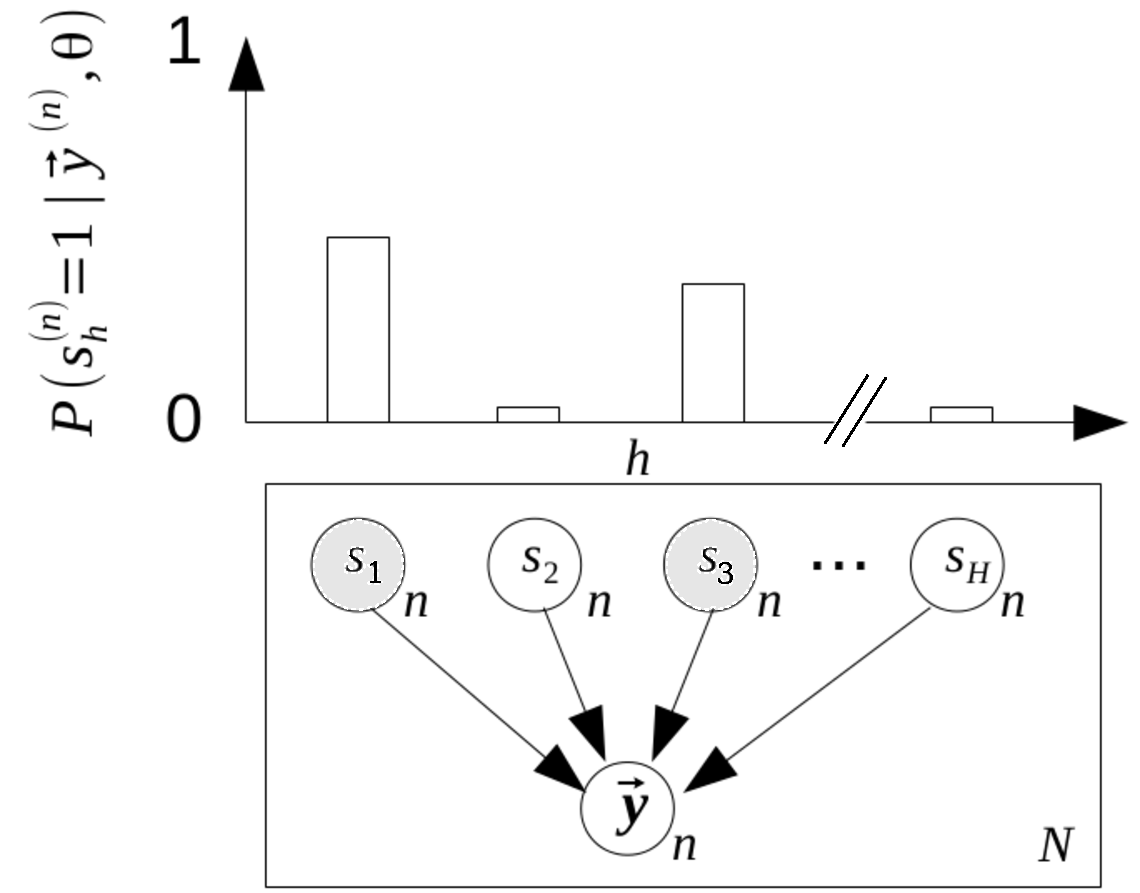
\includegraphics[width=.535\textwidth]{graph-affinity2.pdf}
%\subfigure[Data and converged\\ solution]{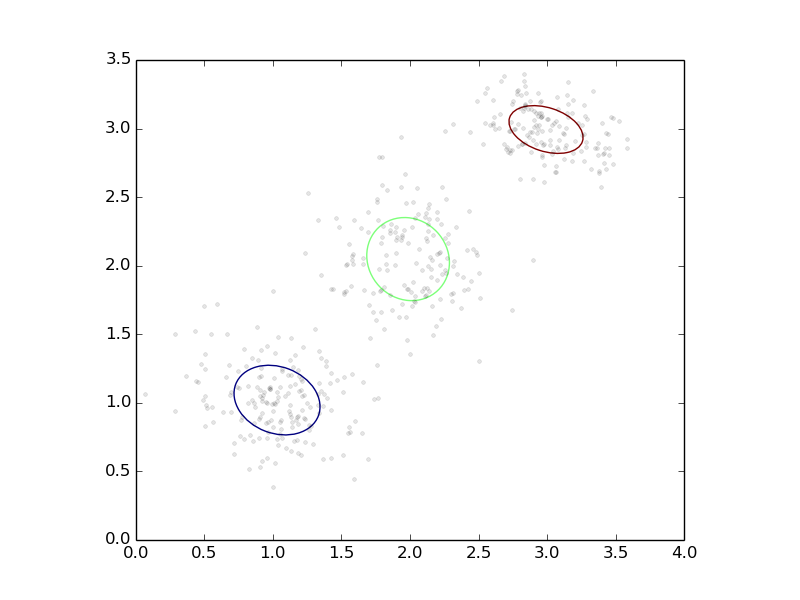
\includegraphics[width=.25\textwidth]{figs/mog/learn-rbf-h2/040.png}}
%\subfigure[GP regression\\ function]{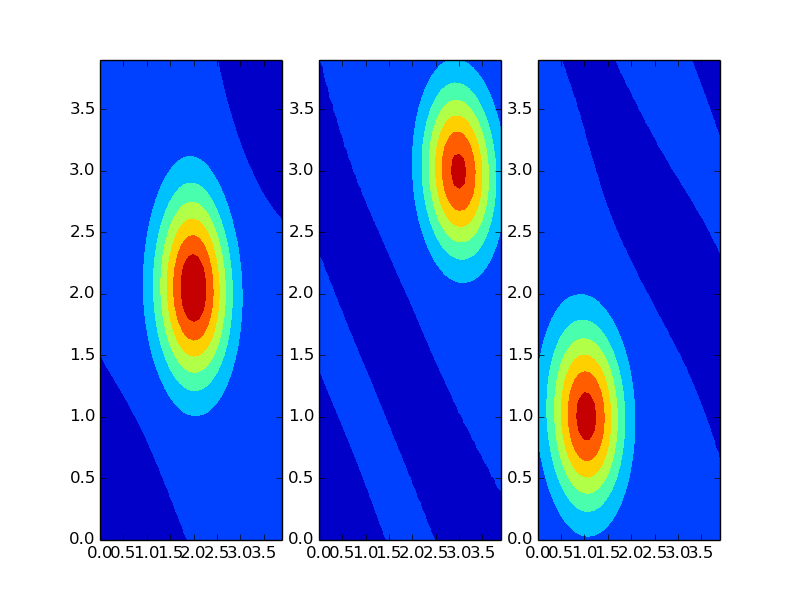
\includegraphics[width=.21\textwidth]{figs/mog/learn-rbf-h2/GP_pred_40.png}}\\
%\centerline{\fbox{This figure intentionally left non-blank}}
\caption{Illustration of the affinity function for selection.
The affinity approximates the marginal posterior probability of each $h=1,\dots,H$ latent variable (top), 
which corresponds to the most relevant variables for a given data point $\vec{y}^{(n)}$ (bottom). 
Here, \rev{the variables $s_1$ and $s_3$ yield high affinity and would thus be considered relevant for $\vec{y}^{(n)}$.} 
%simple graphical model, all $s_{h=1},\dots, s_{H}$ leading to one $\vec{y}^{(n)}$, some plot of marginal posterior, a few are "high" and thus selected?
}\label{fig:graph-affinity}
\end{center}
\end{figure}
%\vspace{-.7cm}
%
One way of constructing a selection function %$\mathcal{S}^{(n)}$ 
is by first ranking the latent variables according to an 
\emph{affinity function} $f_h(\vec{y}^{(n)}) : \mathrm{R}^D \mapsto \mathrm{R}$ %^{+}$
which directly reflects the relevance of latent variable $s_h$. 
%
A natural choice for such a function is the one that approximates the marginal posterior probability 
of each variable, e.g.\ we try to learn $f$ as follows:
%
\begin{equation}
\label{eq:affinity}
% remove vector p^:
f_h(\vec{y}^{(n)}) = \hat{p}_h^{(n)} \approx p^{(n)}_h \equiv p(s^{(n)}_h = 1|\vec{y}^{(n)}, \Theta),
\end{equation}
%
%meaning that, for the relevant variables, the marginal posterior probability $p_h$ 
\rev{meaning that the relevant variables will have greater marginal posterior probability $p_h$.}
%exceeds some threshold. %and is closer to zero for the rest. 
See Figure~\ref{fig:graph-affinity} for a simplified illustration. 
%
When the latent variables $s_{h=1}^{(n)}, \dots, s_H^{(n)}$ in the marginal posterior probability $\hat{\vec{p}}^{(n)} = \hat{p}_{h=1}^{(n)},\dots, \hat{p}_H^{(n)}$ are conditionally independent given a data point $\vec{y}^{(n)}$, this affinity function correctly isolates the most relevant variables in the posterior.
%
\rev{To see this, consider the full joint $p(s_1,...s_h \,|\, y,\Theta)$ in the case when a subset of latents has values clamped to zero, i.e., $s_h=0$ for all $h\not\in\II$ (compare Equation\eqref{eq:sel-post}). We can then ask what the overall joint posterior mass is in this case. If we suppose the latents to be conditionally independent, this total mass is given by a product of marginals as follows:
%
\begin{equation}
\label{eq:marginals-product}
% 1st iteration:
%\sum_{\vec{s}\not\in\II, \,s_h=1 \,\forall\, h\in\II}p(s_1,...,s_h \,|\, y, \Theta) = \prod_{h\in\II}p(s_h=1 \,|\, y, \Theta).\\
\sum_{\vec{s}\; \text{with}\; s_h=0 \;\text{for all}\; h\not\in\II} p(s_1,...s_H \, | \, \vec{y}, \Theta) = \prod_{h\not\in\II} (1 - p(s_h=1 \,|\, \vec{y}, \Theta)).
\end{equation} 
%
We want this mass to be as large as possible as its complement is the posterior mass that we discard with our approximation. If the affinity function correctly estimates the marginals $p(s_h=1 \,|\, \vec{y}, \Theta)$, then discarding those $(H-H')$ marginal with lowest values is equivalent to discarding the space with the least posterior mass (compared to discarding w.r.t. all alternative choices with the same number of latents). }
%
%\rev{See \cite{LuckeEggert2010} for more details on this concept.}
Even when this strong assumption does not hold in practice (which is often the case), however,
the affinity can still correctly highlight relevant variables,
and has been empirically shown to be quite effective when dependencies exist (see e.g. source separation tasks in \citep{SheikhEtAl2014}).


%Using these concepts, we define a general selection function to isolate the relevant regions $\Kn$ as follows.
%First, we define $f_h(\vec{y}^{(n)})$ as a function that takes the input of a single data
%point $\vec{y}^{(n)}$ and predicts the probability that the latent variable
%$s_h$ is equal to $1$ for this particular data point, such that each data point
%$\vec{y}^{(n)}$ is associated with an $H$-dimensional vector of predictions
%$\vec{f}(\vec{y}^{(n)}) = (f_1(\vec{y}^{(n)}), \dots, f_H(\vec{y}^{(n)}))$.
%
Next, using all $\hat{p}_{h=1}^{(n)},\dots, \hat{p}_H^{(n)}$  
%approximated marginal posterior probabilities 
from the affinity function 
$\vec{f}(\vec{y}^{(n)}) = (f_1(\vec{y}^{(n)}), \dots, f_H(\vec{y}^{(n)}))$, we define 
 $\gamma\,(\hat{\vec{p}}^{(n)})$ to simultaneously sort the indices of the latent variables in descending order \rev{[of probability $\hat{p}^{(n)}$]} and \textit{reduce} the sorted set to the $H'$ highest (most relevant) variables' indices. % XXX changed rom rebuttal. states' indices. %, (where $H' \ll H$.
To ensure that there is a non-zero probability of selecting each variable per EM iteration, $10\%$ of the $H'$ indices are uniformly chosen from $H$ at random. 
This prevents the possible propagation of errors from $q_{(n)}$ continuously assigning small probabilities to a variable $s_h$ in early EM
iterations. 
\rev{The optimization of $q(n)$ in early iterations of EM starts from randomly initialized $\vec{s}_h$. Thus it is important that selection-based EM does not "get stuck" assigning higher probability values to $s_h$ selected due to an initially high probability value and therefore always be deemed relevant. Thus to avoid this, we randomly select a few extra hidden indices $H' + .10\times H'$ to give the algorithm an opportunity to evaluate possibly unused variables (those initialized with small probability values) which are actually relevant for $\vec{y}^{(n)}$.}
%
$\gamma(\hat{\vec{p}}^{(n)})$ thus returns the $H'$ selected variable indices $I$ deemed by the affinity to be relevant to the $n$th data point.
%
%(i.e. all $h=1,\dots,H'$ latent variables sorted by estimated relevance).
%
%of the indices $I$ corresponding
%to the highest probability states that $\vec{s}^{(n)}=1$ 
%s a function of each
%$\vec{s}^{(n)}$ that returns a sorted and reduced set of indices $I$ corresponding
%to the highest probability states that $\vec{s}^{(n)}=1$ (output from $\vec{f}(\vec{y}^{(n)})$).
%In other words, $\gamma(\vec{s}^{(n)})$
%sorts all $h,...,H$ of the $s_h^{(n)}$ variables in descending order of estimated relevance.
%
Finally, using the indices $I$ from $\gamma$, we define $\mathcal{I}(I)$ to return an 
$H'$-dimensional subset of selected relevant latent states $\Kn$ for each data point $\vec{y}^{(n)}$. 
%
All `non-relevant' variable states $s_h$ for all variables $h\not\in I$ are effectively set to $0$ in Equation~\eqref{eq:sel-post} 
by not being present in the state set $\Kn$.
\rev{For example, let's say that there are five $s_h$, where $h\in \{1,...,5\}$. We consider the case where only $s_1$   and $s_2$   are selected.  The $\mathcal{I}$ function will then return zeros for $s_3$, $s_4$, and $s_5$, but will  return both allowed possibilities $0$ or $1$ for $s_1$ and $s_2$. Thus a valid setting for the entire vector $\vec{s}$ can be $\vec{s}=[0 1 0 0 0]$, but not $\vec{s}=[0 1 1 0 0]$.}
%to $0$, and returns the set of $H'$ selected relevant latent states' indices $\Kn$.
% with the "non-relevant" variables set to $0$ ($\mathcal{K}_n = \{\vec{s}^{(n)}\,|\,\mbox{for all}\ h\not\in I:\ s_h=0 \}$).
%
%for $K_n$ ... $\mathcal{I}(s) = K_n$ takes a given I, makes $K_n$, basically
%what that math says, but a function that does it
%takes subset of the H variables, produces a subset where everything NOT in subset is set to 0 ... say where s comes from
%We define $\mathcal{K}_n$ as $\mathcal{K}_n = \{\vec{s}\,|\,\mbox{for all}\ h\not\in I:\ s_h=0 \}$ where $\mathcal{I}$ contains the indices of the latents estimated to be most relevant for $\vec{y}^{(n)}$.
%

Using $\vec{f}$, $\mathcal{I}$, and $\gamma$, we can define a 
\emph{selection function} $\mathcal{S}: \mathrm{R}^D \mapsto 2^{ \{1,\dots,H \}}$ 
to select subsets $\mathcal{K}_n$ per data point $\vec{y}^{(n)}$.   
Again, the goal is for the states $\Kn$ to contain most of the probability mass
$\prob{\vec{s}}{\vec{y}}$ and to be significantly smaller than the entire
latent space.  
%
The \textit{affinity based selection function} to obtain the set of states $\Kn$ can be expressed as
%
\vspace{-.1cm}
\begin{equation}\label{eq:sel-func}
\mathcal{S}(\vec{y}^{(n)}) \;=\; \mathcal{I} \left[  \gamma \left[ \vec{f}(\vec{y}^{(n)}) \right]  \right] \;=\; \mathcal{K}_n.
\end{equation}
%
\rev{To summarize, the main task is to formulate a general data-driven function to identify relevant latent variables and to select the corresponding set of states
$\Kn$. 
This is performed using GP regression in order to compute the truncated posterior Equation \eqref{eq:sel-post} on the reduced support $\Kn$.
With the combined effort of the above utility functions, we have concisely defined the function $\mathcal{S}(\vec{y}^{(n)})$ in Equation \eqref{eq:sel-func} to perform this selection.}

% MOVED PART ABOUT SELECTION TO NEXT S$EC 

%Using such subsets $\mathcal{K}_n$, Equation~\eqref{eq:sel-post} results in good approximations to the full posteriors.
%redundant: When the set $\Kn$ fulfills the above property of containing the indices of the states with concentrated posterior mass, Equation~\eqref{eq:sel-post} is a good approximation of the full posterior.

\subsection{Inference in EM with selection}
%
%As a meta algorithm, ET selects the $\Kn$ subspace prior to every EM iteration.
In each iteration of EM, the following occurs: 
prior to the E-step, the selection function $\Ss(\vec{y}^{(n)})$ in \eqref{eq:sel-func} is computed to select the most relevant states $\Kn$, 
which are then used to compute the truncated posterior distribution $q_n(\vec{s})$ in \eqref{eq:sel-post}.
The truncated posterior can be computed using any standard inference method, 
%posterior distribution by computing the true posterior on the truncated space $q_n(\vec{s})$~\eqref{eq:sel-post}.
%With the truncated posterior $q(\vec{s})$, inference can be performed using any standard method, 
such as exact inference or e.g. Gibbs sampling from $q(\vec{s})$  %for a further approximation. % sampling approximation of the truncated posterior.
if inference is still intractable or further computational accerleration is desired.
The result of the E-step is then used to update the model parameters \rev{with maximum likelihood} in the M-step. 

% To summarize, in each iteration of EM, the following occurs: 
%prior to the E-step, the selection function $\Sh$~\eqref{eq:sel-func} is computed to select the most relevant states $\Kn$, 
%which are then used to compute the truncated posterior distribution $q(\vec{s})$~\eqref{eq:sel-post}.
%This result is then used to calculate the model parameter update equations in the M-step. 


\section{GP-Select}
\label{gp-select}
%
%In this work we generalize the above approach, where instead of defining $\Sh$
%by hand, we propose that $\Sh$ be learned in a black-box fashion based on the
%data.
In previous work, the selection function $\mathcal{S}(\vec{y}^{(n)})$ 
was a deterministic function derived  individually for each model 
%AG: that's WAY overkill :)
%has been a manually-derived deterministic function constructed based on the structure of the considered model by hand 
\citep[see e.g.][]{SheltonEtAl2011, SheltonEtAl2012, DaiLucke2012a, DaiLucke2012b,
BornscheinEtAl2013, SheikhEtAl2014, SheltonEtAl2015}, \rev{specific examples of which will be shown in Section 5.1}.
%
We now generalize the selection approach:  %for inference in graphical models
instead of predefining the form of $\Ss$ for variable selection, we want
to learn it in a black-box and model-free way based on the data.
%
We learn $\Ss$  using Gaussian process (GP) regression
\citep[e.g.][]{RasmussenGPbook}, which is a flexible nonparametric model 
and scales cubicly\footnote{If the scaling with $N$ is still too expensive, an incomplete Cholesky approximation is used, with cost linear in $N$ and quadratic in the rank $Q$ of the approximation (see Section~\ref{invec} for details).} with the number of data points $N$ but linearly with the number of latent variables $H$.  
%
%Thus, with the previously defined concepts, we can express the Gaussian process model for the posterior marginal probability that $s_h^{(n)}=1$:
%generative story for a single latent variable $s_h$ as:
%
% TODO REMOVE XXX
%\begin{align}\label{eq:gen-story}
%f_h(\vec{y}^{(n)}) \sim \text{GP}\left(0, \, k(\cdot,\cdot) \right), \,\,\,
%p_h^{(n)} \sim f(\vec{y}^{(n)}) + \epsilon^{(n)}, \\
%\text{and}\quad \epsilon^{(n)} \sim \mathcal{N}(0,\sigma^2_{noise})
%\end{align}
%
%
%TODO put in reasons GPs are awesome!! XXX 
We define the affinity function $f_h$ as being drawn from a Gaussian process model: 
$f_h(\vec{y}^{(n)}) \sim \text{GP}\left(0, \, k(\cdot,\cdot) \right)$, where $k(\cdot, \cdot)$ is the covariance kernel, 
which can be flexibly parameterized to represent the relationship between variables.
%flexibly govern the representation of the relationship between variables.
Again, we use $f_h$ to approximate the marginal posterior probability $p_h$ that $s_h^{(n)}=1$.
%
A nice property of Gaussian processes is that the kernel matrix $K$ need only be computed once (until the kernel function hyperparameters are updated) 
to approximate $p_h^{(n)}$ for the entire $H\times N$ set of latent variables $\vec{S}$.
%the marginal posterior probability

% DO NOT EVEN USE: and $\sigma_{noise}^2$ is the degree of Gaussian noise on the function $f_h$.
Thus, prior to each E-step in each EM iteration, within each calculation of the selection function, we calculate the affinity  using a GP to regress the expected values of the latent variables $\langle \vec{S} \rangle$ onto the observed data $\vec{Y}$.  
Specifically, we train on $p_h$ from the previous EM iteration (where $p_h$ is equal to $\langle s_h \rangle$), for 
training data of 
%$\mathcal{D} = \{ (\vec{y}^{(n)}, \langle\vec{s}_{\text{prev-it}}\rangle^{(n)}_{q(\vec{s})}) | n = 1,\dots, N \}$.
$\mathcal{D} = \{ (\vec{y}^{(n)}, \langle\vec{s}^{(n)}\rangle_{q}) | n = 1,\dots, N \}$, 
where we recall that $q_{n}(\vec{s}^{(n)})$ is the approximate posterior distribution for $\vec{s}^{(n)}$ in Equation~\eqref{eq:sel-post}.
%
%output of the previous iteration of the % EM parameter inference algorithm, $q(\vec{S})$, or rather, the expectations of
%This means that in the very first EM iteration contains no actual information from the posterior distribution, and 
In the first EM iteration, the expectations $\langle\vec{s}^{(n)}\rangle_{q}$ are initialized randomly;
in each subsequent EM iteration, the %true
expectations w.r.t. the $\Kn$-truncated posterior $q(\vec{s})$ are used. 
The EM algorithm is run for $T$ iterations and the hyperparameters of the kernel are optimized by maximum likelihood every $T\ast$ EM iterations.

For each data point $n$ and latent variable $h$ we compute the predicted mean of the GP by leaving 
this data point out of the training set and considering all others, which is called leave-one-out (LOO) prediction.
It can be shown that this can be implemented efficiently \citep[see Section 5.4.2 in ][]{RasmussenGPbook}, 
and we use this result to update the predicted affinity as follows:
%
%We compute the predictive mean for of the predictive probability defined by the GP regression model \comm{(???)} by using
%leave-one-out (LOO) prediction -- the training set consists of $n= 1, \dots,N \backslash n'$ for all $n'=1,\dots, N$.
%In each latent variable $h$ and each data point $n$, the LOO predictive mean is
%
\vspace{-.2cm}  % (*1)
\begin{equation}\label{eq:gp-loo}
%\vec{\mu}^{(n)} \;=\;  \hat{\vec{s}}^{(n)} \;=\;  
%\hat{p}_{h}^{(n)} =   
%p_{h}^{(n)} - \frac{ [ K^{-1} \vec{p}_{h} ]_{nn} }{ [ K^{-1} ]_{nn} }.
\hat{p}_{h}^{(n)} \leftarrow   
% OLD : \langle s \rangle_h^{(n)} 
\langle s_h^{(n)}\rangle_{q_n} - \frac{ [ K^{-1} \langle\vec{s}_{h}\rangle_{q_n} ]_{nn} }{ [ K^{-1} ]_{nn} }.
\end{equation}
%
%which computes the predictions of the GP model using leave-one-out by only computing one kernel matrix inversion (see e.g. Section 5.4.2~\citep{RasmussenGPbook}).
% Namely, it computes a prediction for each $s_{h,t}^{(n)}$ given all variables $\vec{Y}$, where each predicted marginal probability 
%$\hat{s}_h$ represents the GP's characterization of the relationship between the two.
%
Equation~\eqref{eq:gp-loo} can be efficiently implemented for all latent variables $h=1,\dots,H$ and all data points $n=1,\dots,N$ using matrix operations, thereby requiring only one kernel matrix inversion for the entire dataset.
%
%%%%% The idea now is to use these predictions for preselection of relevant latent variables in the EM fashion described earlier. %, we will compute equations~\eqref{eq:loo-gp} in every EM iteration.%, prior to each E-step.
%%%%% Our approach deviates however from classic EM [with preselection]: prior to each E-step we compute GP-selection in Equation~\eqref{eq:gp-sel-
%%%% We are not interested in the actual GP prediction, only in the relative size of each $\hat{s}_h^{(n)}$, which indicates how relevant variable $h$ is to $\vec{y}^{(n)}$.
%%%%% Specifically, we use the prediction size to select which subset of latent variables from $H$ are relevant for a given data point $\vec{y}^{(n)}$:
%
%

Substituting Equation~\eqref{eq:gp-loo} for $\vec{f}$ in the affinity based selection function~\eqref{eq:sel-func} 
\rev{, $$\mathcal{S}(\vec{y}^{(n)}) \;=\;   \mathcal{I} \left[  \gamma \left[ \langle s_h^{(n)}\rangle_{q_n} - \frac{ [ K^{-1} \langle\vec{s}_{h}\rangle_{q_n} ]_{nn} }{ [ K^{-1} ]_{nn} } \right]  \right] 
\;=\; \mathcal{I} \left[  \gamma \left[ \vec{f}(\vec{y}^{(n)}) \right]  \right] 
\;=\; \mathcal{K}_n$$} 
we call the entire process \textit{GP-select}. An outline is shown in Algorithm 1.

%Using LOO prediction leads to the following expression of the \textit{GP selection function} for the $n$th data point:
%
% TODO REMOVE THIS TOO XXX 
%\vspace{-.1cm}      % (*2)
%\begin{equation}\label{eq:gp-sel-func}
%\mathcal{S}(\vec{y}^{(n)}) \;=\; \mathcal{I} \left[ \gamma \left[ \hat{\vec{s}}^{(n)} \right] \right],
%\end{equation}
%
%which specializes Equation~\eqref{eq:sel-func}.
%
%%% where $\gamma(\cdot)$ is a function that sorts the $s_h$ variables in descending order and gives the corresponding indices.
%%% This selection function $\mathcal{S}(\vec{y}^{(n)})$ aids with dimensionality selection -- it provides a ranking of the $H$ latent variable indices, from which we choose  $h,\dots, H' < H$ for the subset $\mathcal{K}_n$ per data point that we will use for inference.
%%% Particularly, we can use this subset $\mathcal{K}_n$ to define the support for the reduced posterior distribution $q_n(\vec{s}, \Theta)$, and perform inference more efficiently with far fewer further approximations.
%%% With no tricks, we we can draw samples from the true posterior of these variables and, given the reduced size of the posterior space, sampling methods can perform efficiently.
%%% Or depending on the size of $\mathcal{K}_n$ we can calculate the posterior $q_n$ exactly for exact inference in this reduced space.

%%% For additional computational efficiency in large latent spaces or when no analytic solution is possible, the expectations with respect to the posterior can be approximated by sampling in the GP-selected latent space.
%In order to compute/update model parameters, expected values with respect to the posterior are the main computations necessary, i.e.:
%\begin{align}\label{eq:sel-samp}
%\langle g(\vec{s}) \rangle_{p(\vec{s}\,|\,\vec{y}^{(n)},\Theta)} \;  & \approx \; \langle g(\vec{s}) \rangle_{q_n(\vec{s};\Theta)}\\
%\; & \approx \;  \frac{1}{M}\sum_{m=1}^{M}g(\vec{s}^{(m)})
%\phantom{iii}\mbox{with}\phantom{iii}\vec{s}^{(m)}\sim q_n(\vec{s};\Theta),
%\end{align}
%

% TODO PUT ALGO HERE XXX
\begin{algorithm}
\caption{GP-Select to accelerate inference in Expectation Maximization}
\label{alg:gp-select}
\begin{algorithmic}

\FOR{EM iterations $t=1,\dots,T$}\STATE{%\vspace{-.4cm}   
\rev{initialize all latent variables expectations $\langle s_h^{(n)}\rangle_{q_{n,t}}$}
    \FOR{data point $n=1,\dots, N$}
    \STATE{
    compute affinity of all latent variables $\hat{\vec{p}}_t^{(n)}$: Eq. \eqref{eq:gp-loo}\\
%2. sort and reduce indices to $H'$\\
 %   2.2. include uniformly chosen indices\\
    compute subset of relevant states $\Ss$: Eq. \eqref{eq:sel-func}\\ % get $\Kn$ 
%3. puke out reduced set of latent states $\Kn$ to use to calculate posterior distribution in E-step\\
    compute truncated posterior $q_{n,t}(\vec{s}^{(n)})$ in E-step: Eq. \eqref{eq:sel-post}\\ % on reduced set $\Kn$
    update model parameters \rev{in M-step, e.g. as in Sec. 5.1}\\ 
    store $\langle s_h^{(n)}\rangle_{q_{n,t}}$ for $\vec{p}^{(n)}$ in EM iteration ${t+1}$\\
%\langle \vec{s} \rangle^{(n)}_{q_{t}(\vec{s})}$ 
    }\ENDFOR\\%\vspace{-.2cm}
    optimize kernel hyperparams every $T\ast$ EM iterations
}%\vspace{-.2cm}
\ENDFOR
\end{algorithmic}
\end{algorithm}

\iffalse
 Optimization of the model parameters in EM continues in the standard EM-style format as described earlier: the
M-step computes the model parameters based on these subsets of $\Kn$ 
(the indices of the $H' < H$ 'most relevant' states) 
to approximate the posterior distribution shown in Equation~\eqref{eq:sel-post}.

Our approach functions as a meta algorithm to the EM algorithm by incorporating latent variable selection.
A summary of the process is as follows:
We identify the relevance of each latent (binary) variable $h\dots H$ by approximating its marginal posterior probability using GP regression. 
When this exceeds some threshold, the variable likely contains relevant information and its index should be in the $H'$-dimensional set $K_n$.
%Furthermore, when all $H$ latents in the marginal posterior are conditionally independent, the affinity function $f_h$ is indeed the correct way to isolate the most relevant variables and is a useful approximation even when dependencies exist.%We (approximately) learn the marginal posteriors using GP regression. 
We use the expectations of $\vec{s}$ from the previous EM iteration as the target in the subsequent GP regression, which will give the marginal posterior approximation to guide the variables selected for inference in the next EM iteration.
\fi

\section{Experiments}
\label{exps}
%
% XXX UNDER CONSTRUCTION XXX
We apply our GP-select inference approach to five different probabilistic generative models.
%
First, we considered three sparse coding models (binary sparse coding,
spike-and-slab, nonlinear spike-and-slab), where the relationship between the
observed and latent variables is known to be complex and nonlinear.
%
Second, we apply GP-select to a simple Gaussian mixture model,
to both provide functional intuition of approach and to explicitly visualize the form of the learned regression function.
%We find that even for a simple model, it can be be essential to learn a nonlinear mapping.
%this matches well with our expectations for the model, and again reveals that it may be essential to learn a nonlinear mapping.
%
Finally, we apply our approach to a recent hierarchical model for translation invariant occlusive components analysis
\citep{DaiLucke2012a,DaiEtAl2013,DaiLucke2014}.

% TODO define composition kernel 

\subsection{Sparse coding models}
\label{sec:sparse-coding}
%
\rev{Many types of natural data are composed of potentially many component types but any data point often only contains a very small number of this potentially large set of components. For the introductory example of toys on the nursery floor, for instance, there are many different toys that can {\em potentially} be in a given image but there is only a typically relatively small number of toys {\em actually} appearing in any one image.
Another example is a sound played by a piano at a given time $t$. While the sound can contain waveforms generated by pressing any of the $88$ piano keys, there are only relatively few keys (typically much smaller then ten) that actually generated the sound. Sparse Coding algorithms model such data properties by providing a large number of hidden variables (potenial data components) but assigning non-zero (or significantly different from zero) values only to a small subset of components (the acturally appearing components). 
%%% TODO citations below %%%%
Sparse coding algorithms are typically used for tasks such as denoising \citep{EladAharon2006,MairalEtAl2009}, inpainting \citep{MairalEtAl2009, MairalEtAl2009b,TitsiasGredilla2011}, classification 
\citep[][e.g. MNIST data set \emph{http://yann.lecun.com/exdb/mnist/}, the flowers data set \emph{http://www.robots.ox.ac.uk/$\sim$vgg/data/flowers/}]{MNIST,TitsiasGredilla2011,RainaEtAl2007}, transfer learning \citep{RainaEtAl2007}, collaborative filtering \citep{TitsiasGredilla2011} and are important models for neuro-sensory processing \citep[][and many more]{OlshausenField1997,ZylberbergEtAl2011,BornscheinEtAl2013,SheikhEtAl2014}.}
%
%We hereby consider an object to be the same even if it appears at different positions or at different intensity levels. The property that there are only few components in any given data point can be modeled using the concept of sparsity, the property that a component’s identity is unchanged by it appearing intensity, position or other types of transformations can be modeled using mathematical models of intensity and transformation invariances.
%
A variety of sparse coding models have been successfully scaled to high-dimensional latent spaces with use of selection~\citep{HennigesEtAl2010, BornscheinEtAl2013, SheikhEtAl2014} or the use of selection combined with Gibbs sampling~\citep{SheltonEtAl2011, SheltonEtAl2012, SheltonEtAl2015} inference approaches. \rev{Latent variables were hereby selected using selection functions that were individually defined for each model.}
%
In order to demonstrate our method \rev{of autonomously learned selection functions}, we consider three of these
 sparse generative models, and perform inference in EM with our GP-select approach instead of a hand-crafted selection function.
\rev{The models are relevant for different tasks such as classification (e.g., binary sparse coding), source separations and denoising (linear spike-and-slab sparse coding) or sparse encoding and extraction of interpretable image components (nonlinear sparse coding). 
Note that when it is obvious from context, we drop the notation referring to each $n$ data point independently in order to make the the equations more concise.}

The models \rev{and their parameters} are:
%
%\begin{enumerate}
\begin{description}
%
%%% BSC %%%
\item[\textbf{A.}] \textit{Binary sparse coding}:
%
\vspace{-.1cm}
\begin{align}
\text{latents: } \,\,\,         \vec{s} &\sim Bern(\vec{s} | \pi) = \disT\prod_{h=1}^H \pi^{s_h} \big( 1 - \pi \big)^{1-s_h}\nonumber \\
\text{observations:  }\,\,\,    \vec{y} &\sim \mathcal{N}(\vec{y}; W\vec{s}, \sigma^2\One)\nonumber \\ 
\rev{\text{parameters: }} \,\,\,  % W update
\disT{}\rev{W} &= \big( \sum_{n=1}^{N} \vec{y}^{(n)} \E{\vec{s}\,}^T_{q_n} \big)\ \big( \sum_{n=1}^{N} \left< \vec{s}\,\vec{s}^{\,T}\right>_{q_n}\big)^{-1}\, \nonumber\\
% sigma 
\rev{\disT{}\sigma^2} &= \frac{1}{ND} \sum_{n} \left< \left|\left| \vec{y}^{(n)} - W \, \vec{s} \right|\right|^2 \right>_{q_n}\hspace{-2mm}\nonumber\\
% pi
\rev{\pi} &= \frac{1}{N} \sum_{n}\, |\big< \vec{s} \big>_{q_n}|,\:\:\mbox{\small where}\:|\vec{x}|=\frac{1}{H}\disS\sum_{h}x_h \nonumber
\end{align}
%
where $W \in \mathrm{R}^{D \times H}$ denotes the components / dictionary elements and $\pi$ parameterizes the sparsity (see e.g.~\citep{HennigesEtAl2010}).
%\
% XXX 
%\vspace{.4cm}
%
%%% spike and slab %%%
\item[\textbf{B.}] \textit{Spike-and-slab sparse coding}:
\vspace{-.2cm}
\begin{align}
\text{latents: } & \,\,\,\vec{s} = \vec{b}\odot\vec{z}
\text{\quad}\mathrm{where\;}\quad \vec{b}\sim Bern(\vec{b} | \pi)
\:\mathrm{and} \:
\vec{z} \sim \mathcal{N}(\vec{z};\,\vec{\mu} , \Sigma_h)\nonumber\\
%\sim \odot 
\text{\quad}\text{observations:} & \,\,\, \vec{y} \sim \mathcal{N}(\vec{y}; W\vec{s}, \sigma^2\One)\text{\quad}\text{\quad}\nonumber\\%\label{eq:gsc}
\text{\quad}\text{\quad}\text{\quad}\text{\quad}\text{\quad}\rev{\text{\;\;parameters: }} \,\,\,   %\nonumber\\
%%% GSC JMLR paper M-step eqjuations:
% W update
  &\rev{W} = \frac{\sum_{n=1}^{N} \yVecN \E{\sVec\odot\zVec}^{\TT}_n}
  {\sum_{n=1}^{N} \E{(\sVec\odot\zVec)(\sVec\odot\zVec)^{\TT}}_n } \nonumber\\
%
% pi update
&\rev{\piVec} =
\frac{1}{N}\sum_{n=1}^{N}\E{\sVec}_n \nonumber\\
%
% sigma update
&\rev{\sigma^2} =
    \sum_{n=1}^{N} \Big[\E{(\sVec\odot\zVec)(\sVec\odot\zVec)^{\TT}}_n 
    \ssb -  \E{\sVec\,\sVec^{\TT}}_n \ssb \odot \muVec\muVec^{\TT} \Big] 
    \odot \Big(\sum_{n=1}^{N}\Big[\E{\sVec\,\sVec^{\TT}}_n \Big]\Big)^{-1} \nonumber\\
%
% mu prior update
&\rev{\mu_{pr}}  = \frac{\sum_{n=1}^{N} \E{\sVec\odot\zVec}_n}{\sum_{n=1}^{N}\E{\sVec}_n}  \nonumber\\
%
% sigma prior update
&\rev{\sigma^{2}_{pr}} = \frac{1}{N}\sum_{n=1}^{N}\Big[ \yVecN(\yVecN)^{\TT}
        - W\big[\E{(\sVec\odot\zVec)}_n\E{(\sVec\odot\zVec)}_n^{\TT}\big]W^{\TT}\Big]  \nonumber
\end{align}
where the point-wise multiplication of the two latent vectors, i.e., $(\vec{s}\odot\vec{z})_h = s_h\,z_h$
generates a `spike-and-slab' distributed variable ($\vec{s}\odot\vec{z}$), that has either continuous values or exact zero entries (e.g. \citep{TitsiasGredilla2011,GoodfellowEtAl2013,SheikhEtAl2014}).
% FIXME FIXME FIXME
%
%%% SSMCA %%%
\item[\textbf{C.}] \textit{Nonlinear Spike-and-slab sparse coding}:
\vspace{-.2cm}
%
\begin{align}\label{eq:ssmca}
\text{latents: } & \,\,\,\vec{s} = \vec{b}\odot\vec{z} \nonumber
\quad\mathrm{where}\quad \vec{b}\sim Bern(\vec{b} | \pi)\nonumber\\
\:&\mathrm{and} \:
\vec{z} \sim \mathcal{N}(\vec{z};\,\vec{\mu_{pr}} , \sigma^2) \nonumber\\ %\text{\quad}\text{\quad}\text{\quad}\text{\quad}\text{\quad}\text{\quad}\text{\quad}\text{\quad}\text{\quad}\nonumber\\
 \text{observations:}\,\,\, &\vec{y} \sim \mathcal{N}(\vec{y}; \max_{h}\{s_h\vec{W}_{h}\}, \sigma^2\One)\nonumber\\
%
%
\rev{\text{\quad parameters: }} \,\,\,\nonumber %\,\,\, &\nonumber
% m-step updates
%
% W 
&\rev{\hat{W}_{hd}}   = \frac{\langle s_h y_d \rangle^*}{\langle s_d^2 \rangle^*} 
 \text{\quad}\text{\quad}\text{\quad}\text{\quad}\text{\quad}\text{\quad}
 %\text{\quad}\text{\quad}\text{\quad}\text{\quad}\text{\quad}
% pi%
\text{\quad}\text{\quad}\rev{\hat{\pi}} = \langle \mathbb{I}(s) \rangle  \text{\quad}\nonumber\\
%
% sigma 
&\rev{\hat{\sigma}^2} = \left\langle W_{dh} s_h - y_d^{(n)}\right\rangle^\ast \nonumber\\
%
% mu prior
&\rev{\hat{\mu}_{\pr}} = \langle s_h \rangle^* 
 \text{\quad}\text{\quad}\text{\quad}\text{\quad}\text{\quad}\text{\quad}\text{\quad}
% sigma prior
\rev{\hat{\sigma}^2_{\pr}} = \langle (s_h - \hat{\mu}_{\pr})^2 \rangle^* \nonumber\\
% sigma 
%%%%%&\rev{\hat{\sigma}^2} = \left\langle W_{dh} s_h - y_d^{(n)}\right\rangle^\ast \nonumber\\
%
%
&\rev{\text{Where expectations $\langle \,.\, \rangle^*$ mean:}}\nonumber\\
%
&\rev{\langle f(s) \rangle^\ast} = \sum_n \frac{ \int_s \, p(\vec{s}|\vec{y}^{(n)},\Theta) \, f(\vec{s}) \, \mathbb{I}(\text{h is max}) \, d\vec{s} }
                                       { \int_s \, p(\vec{s}|\vec{y}^{(n)},\Theta) \, \mathbb{I}(\text{h is max}) \, d\vec{s} } \nonumber
\end{align}
%
\rev{where $\mathbb{I}$ is the indicator function denoting the domain to integrate over, namely where $h$ is the maximum.
Using $\langle f(s) \rangle^\ast$ allows for the condensed expression of the update equations shown above.}
The mean of the Gaussian for each $\vec{y}^{(n)}$ is centered at $\max_{h}\{s_h\vec{W}_{h}\}$, where $\max_{h}$ is a nonlinearity that considers all $H$ latent components and takes the $h$ yielding the maximum value for $s_h\vec{W}_{h}$ \citep{LuckeSahani2008,SheltonEtAl2012,BornscheinEtAl2013,SheltonEtAl2015}, instead of centering the data at the linear combination of $\sum_h s_h\vec{W}_h=W\vec{s}$.
%
\end{description}
%\end{enumerate}

In the above models, inference with the truncated posterior \rev{of Equation~\eqref{eq:sel-post} using hand-crafted selection functions} \rev{$\mathcal{S}_h(\vec{y}^{(n)})$} \rev{to obtain the subset of states} \rev{$\Kn$} \rev{[of selected relevant variables} \rev{$\vec{s}(\vec{y}^{(n)})$}\rev{], shown in Equation~\eqref{eq:sel-func},} has yielded results as good as or more robust than exact inference (converging less frequently to local optima than exact inference; see earlier references for details).
For models \textbf{A} and \textbf{C}, the \rev{hand-constructed function approximating} \rev{$\vec{f}(\vec{y}^{(n)})$}\rev{, for substituion in Equation~\eqref{eq:sel-func},} was the cosine similarity between the weights $\vec{W}_h$ (e.g. dictionary elements, components, etc.) associated with each latent variable $s_h$ and each data point $\vec{y}^{(n)}$: 
%
\rev{$\vec{f}(\vec{y}^{(n)})$} \rev{$ = (\vec{W}_{h}^{\mathrm{T}}\,/\,||\vec{W}_{h}||)\,\vec{y}^{(n)}$}.
%, with $\disT ||\vec{W}_{h}||=\sqrt{\sum_{d=1}^D(W_{dh})^2}$.
For model \textbf{B}, \rev{the affinity function constructed} was the data likelihood given a singleton state:
%
\rev{$\vec{f}(\vec{y}^{(n)})$} $= p(\vec{y}^{(n)} | \vec{s}=\vec{s}_h, \Theta)$, 
%
where $\vec{s}_h$ represents a singleton state in which only the entry $h$ is non-zero.
%, and it does not take into account  the probability of the state itself  (i.e., $p(\vec{s}_h\,|\,\Theta)$).
%repeat: We will train GP regression for our flexible selection approach, where, for all models, the targets of the training data is the expected values of the latents.

\rev{The goal of these experiments is to demonstrate the performance of GP-select and the effects/benefits of using different selection functions. To do this, we consider artifical data generated according to each sparse coding model and thus with known ground-truth parameters. As discussed above, we could also apply the sparse coding models using GP-select to other application domains listed, but that is not the focus of these experiments.} 
We generate $N=2,000$ data points consisting of $D=5\times5=25$ observed dimensions and $H=10$ latent components according to each of the models \textbf{A-C}:
%the dataset consists of
$N$ images of randomly selected overlapping 'bars' with varying intensities for models \textbf{B} and \textbf{C}, and additive Gaussian noise parameterized by ground-truth $\sigma^2 = 2$ and we choose $H' = 5$, (e.g. following the spike-and-slab prior). 
On average, each data point contains $2$ bars, i.e. ground-truth is $\pi H = 2$, and we choose $H'=5$. With this choice,
we can select sufficiently many latents for virtually all data points.

%(i.e. ground-truth is $H'=2$, but we allow the selection function to choose $H'=5$ per data point).

For each of the models considered, we run 10 repetitions of each of the following set of experiments: (1) selection using the respective hand-crafted selection function,
(2) GP-select using a linear covariance kernel, (3) GP-select using an RBF covariance kernel, and (4) GP-select using a kernel composed by adding the following kernels: RBF, linear, bias and white noise kernels, which we will term the \emph{composition kernel}.
% XXX
% TODO XXX where the fuck is our code? how was this coded indeed?
% XXX
%silly: The latter has been shown to be particularly adaptive to data, i.e. generally when there is no linear trend in the data, the variance of that kernel would go to zero.
As hyperparameters of kernels are learned, the composition kernel (4) can adapt itself to the data and only use the kernel components required. 
See  \citet[Chapter 4, Secton 4.2.4]{RasmussenGPbook}  for a discussion on  kernel adaptation.
Kernel parameters were model-selected via maximum marginal likelihood every $10$ EM iterations.
%As inference with the hand-crafted selection functions has already been shown to converge to extract ground-truth parameters, we do not explicitly compare with this case.
For models \textbf{A} and \textbf{B}, inference was performed exactly using the truncated posterior~\eqref{eq:sel-post}, but as exact inference is analytically intractable in model \textbf{C}, inference was performed by drawing Gibbs samples from the truncated space \citep{SheltonEtAl2011,SheltonEtAl2012,SheltonEtAl2015}.
%AG: you already made the point below.
%The number of selected latent variables was set to $H'=5$.
%
We run all models until convergence. %these experiments for $30$ EM iterations for models [1] and [3] and for $60$ iterations for model [2].

\begin{figure}[h!]
\begin{center}
% TODO find a way to rearrange the bars in the svg. ugh.
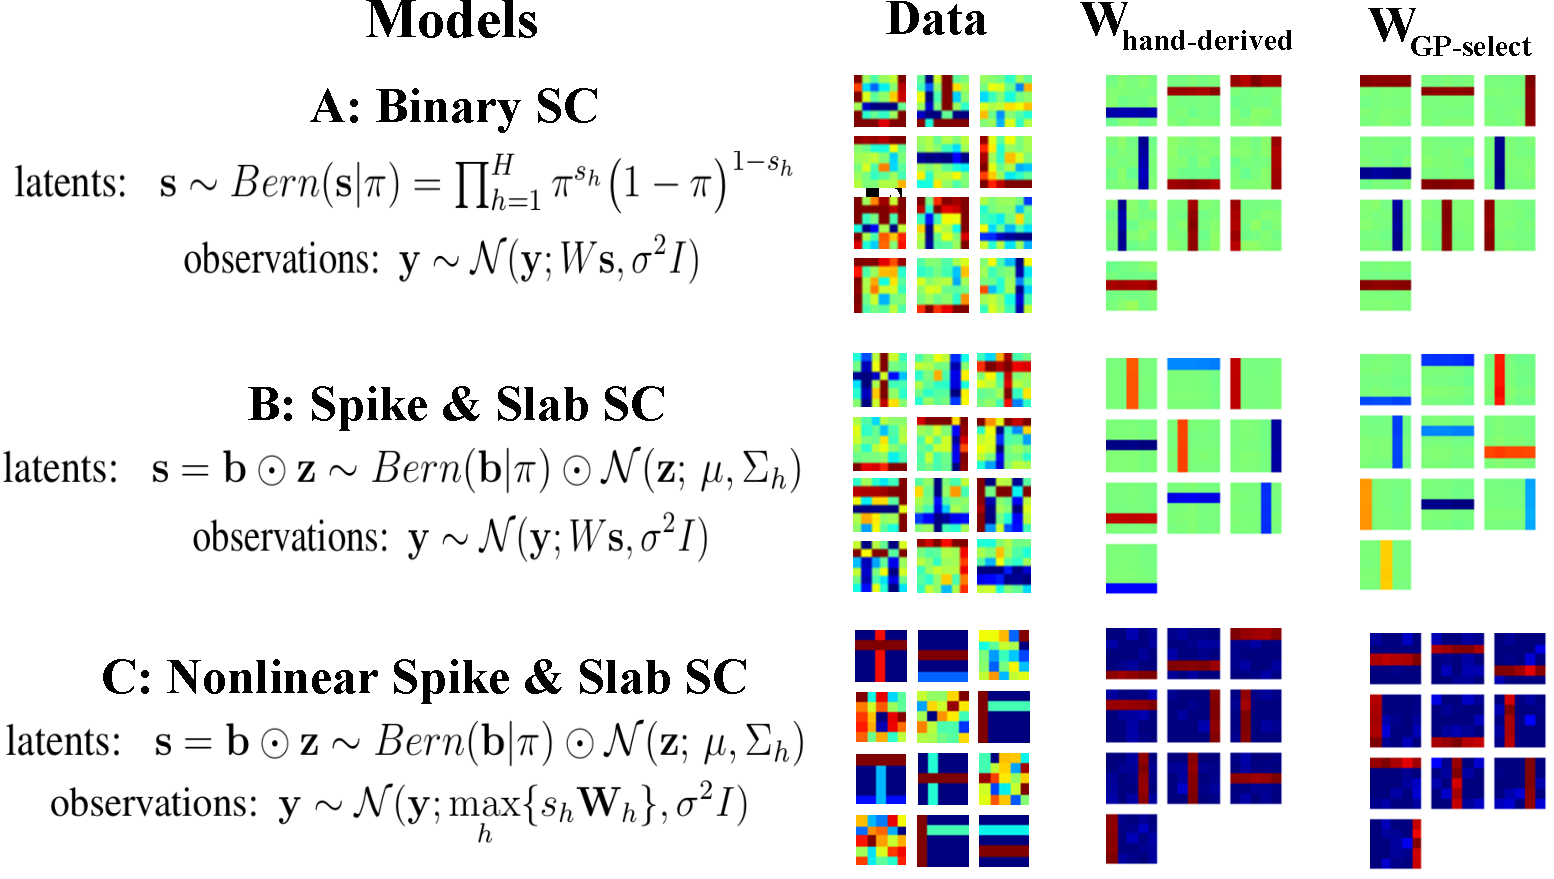
\includegraphics[width=.8\textwidth]{sparsecoding/bars-test_transpose.pdf}%{figs/sparsecoding/bars-test.pdf}
%\subfigure[Data and converged\\ solution]{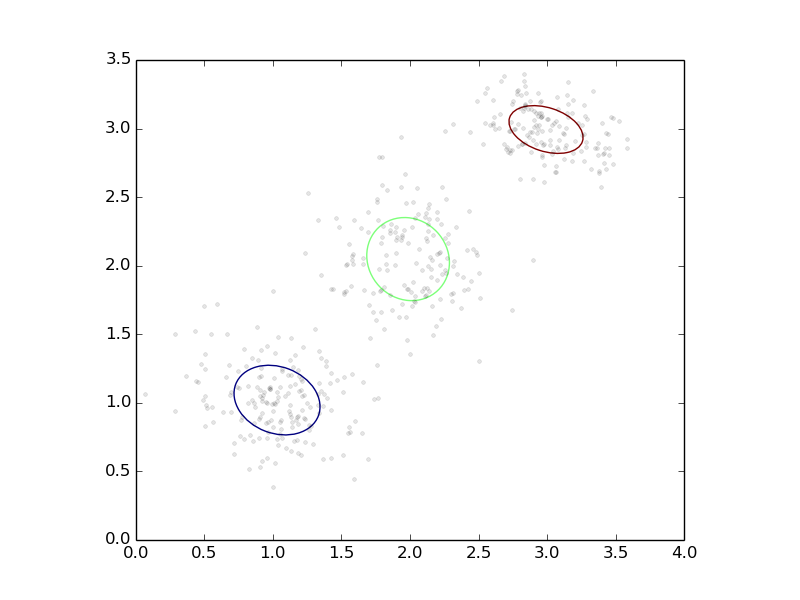
\includegraphics[width=.25\textwidth]{figs/mog/learn-rbf-h2/040.png}}
%\subfigure[GP regression\\ function]{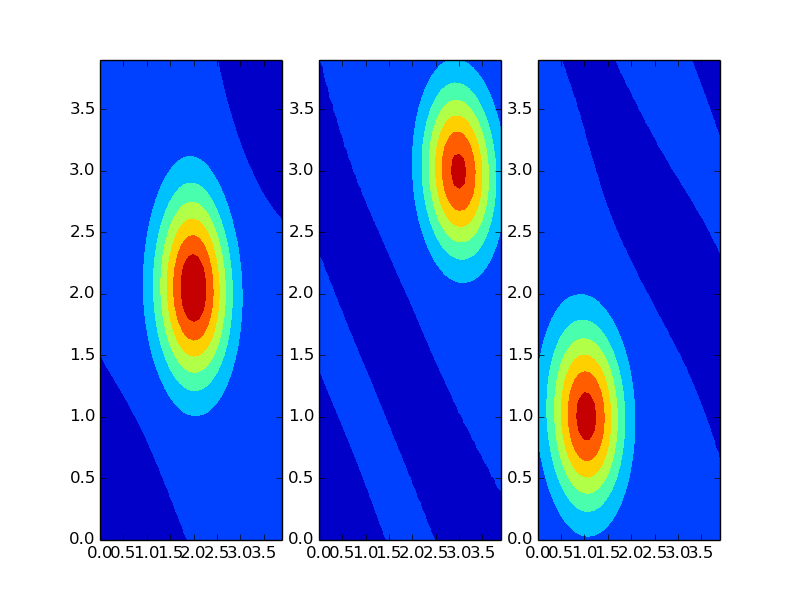
\includegraphics[width=.21\textwidth]{figs/mog/learn-rbf-h2/GP_pred_40.png}}\\
%\centerline{\fbox{This figure intentionally left non-blank}}
\caption{Sparse coding models results comparing GP-select with a successful hand-derived selection function.
Results are shown on artificial ground-truth data with $H=10$ latent variables and $H'=5$ preselected variables for: \textbf{A} Binary sparse coding, \textbf{B} Spike-and-slab sparse coding, and \textbf{C} Nonlinear spike-and-slab sparse coding.
First column: Example data points $\vec{y}^{(n)}$ generated by each of the models.
Middle column: Converged dictionary elements $W$ learned by the hand-crafted selection functions.
Third column: Converged dictionary elements $W$ learned by GP-select with $H'=5$ using the kernel with best performance (matching that of inference with hand-crafted selection function).
In all cases, the model using the GP-select function converged to the ground-truth solution, just as the hand-crafted selection functions did.
}\label{fig:sparse}
\end{center}
\end{figure}

Results are shown in Figure~\ref{fig:sparse}.
In all experiments, the GP-select approach was able to infer ground-truth parameters as well as the hand-crafted function.
For models where the cosine similarity was used (in \textbf{A} and \textbf{C}), GP regression with a linear kernel quickly learned the ground-truth parameters, and hence fewer iterations of EM were necessary.
In other words, even without providing GP-select explicit weights $W$ as required for the hand-crafted function, its affinity function using GP regression~\eqref{eq:gp-loo} learned a similar enough function to quickly yield identical results.
Furthermore, in the model with a less straight-forward hand-crafted function (in the spike-and-slab model of \textbf{B}), only GP regression with an RBF kernel was able to recover ground-truth parameters.
In this case (model \textbf{B}), GP-select using an RBF kernel recovered the ground-truth 'bars' in $7$ out of $10$ repetitions, whereas the hand-crafted function recovered the bases in $8$ instances.
For the remaining models, GP-select converged to the ground-truth parameters with the same average frequency as the hand-crafted functions.
%This suggests difficulty in predicting which kernel will work a priori.

%Hand crafted functions can do as well as exact case, as shown in papers.
%Some sort of kernel can do as well as a selection function engineered by hand.

%AG: where is the experiment for the below?
Finally, we have observed empirically that the composition kernel is flexible enough to subsume all other kernels:
the variance of the irrelevant kernels dropped to zero in simulations.
This suggests the composition kernel is a good choice  for general use. 
%as the composition kernel is flexible enough to adapt to both linear and nonlinear relationships, this supports it as a reasonable general choice.


\subsection{Gaussian mixture model}
%
Next, we apply GP-select to a simple example, a Gaussian mixture model, where the flexibility of the approach can be easily and intuitively visualized.  \rev{Furthermore, the GMMs flexibility allows us to explicitly visualize the effect of different selection functions.
A demonstration and code for the GMM application is shown in \citep{GP-selectNotebook16}.}
%To illustrate the idea and benefit of this approach, we consider a simple motivating example: the problem setting posed by Gaussian mixture models.

The model of the data likelihood is
%
\vspace{-.2cm}
\begin{equation}\label{eq:mog}
p(\vec{y}^{(n)} | \vec{\mu_c}, \vec{\sigma_c}, \vec{\pi}) = \sum_{c=1}^{C} \mathcal{N}(\vec{y}^{(n)}; \vec{\mu_c}, \vec{\sigma_c}) \, \pi_c,
\end{equation}
%
where $C$ is the number of mixture components; the task is to assign each data point to its latent cluster.
%%%  infer from which cluster each data point originates.
%%% The latent distribution gives the prior probability of a data point coming from each cluster $c$, $p(s^{(n)} = c | \pi) = \pi_c$, and data from the $c$th cluster are distributed according to the $c$th component, $p (\vec{y}^{(n)} | s^{(n)} = c) = p_c(\vec{y}^{(n)})$.
%%% Once a data point $\vec{y}^{(n)}$ is observed, the posterior probability distribution for the cluster it belongs to is
%%
%% \vspace{-.15cm}
%%\begin{equation}\label{eq:mog-post}
%% p(s^{(n)} = k | \vec{y}^{(n)}) = r_c^{(n)} = \frac{p_c(\vec{y}^{(n)})\, \pi c}{\sum_c^{C} p_c(\vec{y}^{(n)}) \, \pi c},
%% \end{equation}
%

The training data used for GP regression was $\mathcal{D} = \{ (\vec{y}^{(n)}, \langle s_h^{(n)}\rangle_{q_n}) | n = 1, \dots, N \}$, where the targets were the expected cluster responsibilities (posterior probability distribution for each cluster) for all data points, $\langle s_h\rangle_{q}$, and we use one-hot encoding for cluster identity.
With this, we apply our GP-select approach to this model, computing the selection function according to Equation~\eqref{eq:sel-func} with affinity $f$ defined by GP regression~\eqref{eq:gp-loo} 
and following the approximate EM approach as in the previous experiments.
%%% by applying Equation~\eqref{eq:gp-sel-func} to compute the posterior distribution in~\eqref{eq:mog-post}.
%
%Although the increase in computational efficiency by selecting a reduced set of $K$ mixture components would only be e number of clusters considered to be in the data is very large,
% Depending on the data
In these experiments we consider two scenarios for EM learning of the data likelihood in Equation~\eqref{eq:mog}: GP-select with an RBF covariance kernel and a linear covariance kernel.  
% XXX new from rebuttals:
We do not include the composition kernel suggested (based on experiments) in Section 4.1, as the goal of the current experiments is to show the  effects of using the 'wrong' kernel. These effects would further support the use of the flexible composition kernel in general, as it can subsume both kernels considered in the current experiments (RBF and linear).
%, and the composition kernel used in the sparse coding experiments (RBF, linear, bias, and white).
%
%, where $r_c^{(n)}$ is the responsibility of the $k$th Gaussian for the $n$th data point, $y^{(n)}$.
%%% With this, we calculate the GP predictions following Equations~\eqref{eq:gp-sel-func} and use the prediction size to select which $c$ clusters to include in the normalization in the calculation of the responsibilities $\vec{r}$ (where $\vec{S}$ is substituted with $\vec{r}$).

To easily visualize the output, we generate $2$-dimensional observed data ($\vec{y}^{(n)} \in \mathrm{R}^{D=2} $) from $C=3$ clusters -- first with randomly assigned cluster means, and second such that the means of the clusters lie roughly on a line.
In the GP-select experiments, we select $C' = 2$ clusters from the full set,
and run $40$ EM iterations for both kernel choices (linear and RBF).
Note that for mixture models, the notation of $C'$ selected clusters of the $C$ set is analogous to the $H'$ selected latent variables from the $H$ full set, as described in the non-mixture model setting, and the GP-select algorithm proceeds unchanged.
%%% the indices for which are contained in $\mathcal{K}_n$),
We randomly initialize the variance of the clusters $\vec{\sigma_c}$ and initialize the cluster means $\vec{\mu_c}$ at randomly selected data points.
Results are shown in Figure~\ref{fig:mog}.

\begin{figure*}[t]
\begin{center}
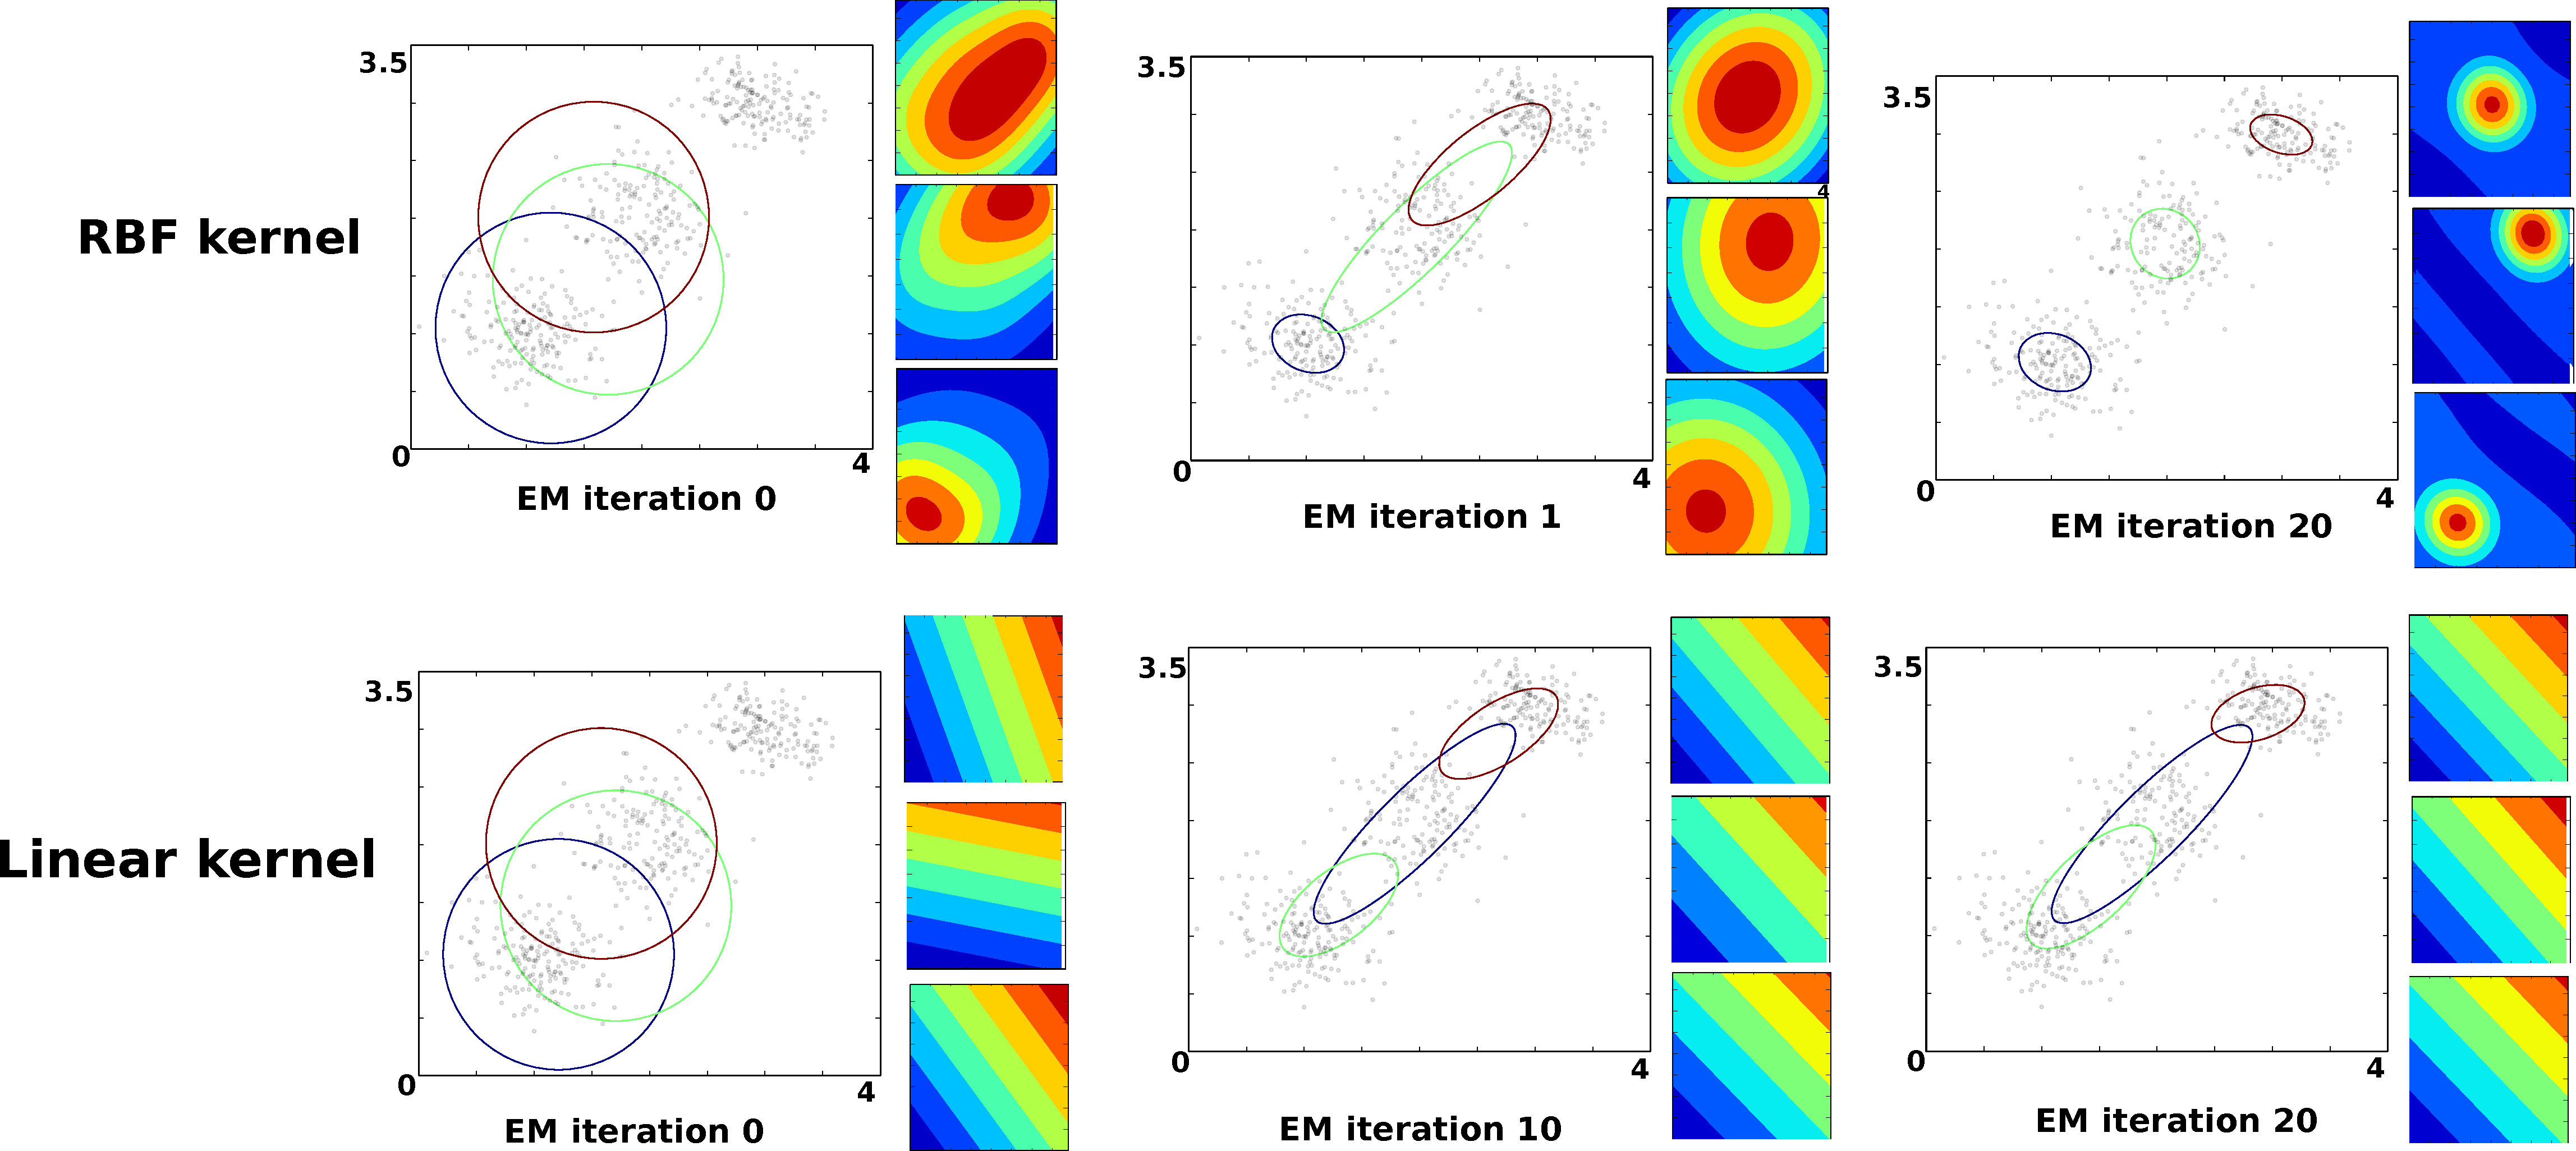
\includegraphics[width=1\textwidth]{mog/mog_labels2.pdf}%{figs/mog/mog.pdf}
\caption{Gaussian mixture model results using GP-select (selection of $C'=2$ in a $C=3$ class scenario) for inference.
Progress of the inference is shown using (row one) an RBF covariance kernel in the regression, and (row two) a linear covariance kernel.
For each iteration shown, we see (1) the observed data and their inferred cluster assignments and (2) the $C$ corresponding GP regression functions learned/used for GP-select in that iteration. Different iterations are pictured due to different convergence rates. As shown, inference with GP-select using a linear kernel is unable to assign the data points to the appropriate clusters, whereas GP-select with an RBF kernel succeeds.}\label{fig:mog}% iterations RBF: 0, 1,, 20, LIN: 0,10, 20
\end{center}
\end{figure*}

%%% XXX NOT TRUE: When the data are allowed to have clusters with means scattered about, both kernels used for GP-selection inference can find the optimal cluster assignments of the data.
With cluster parameters initialized randomly on these data, the linear GP regression prediction cannot correctly assign the data to their clusters (as seen in Figure~\ref{fig:mog}\textbf{B}), but the nonlinear approach successfully and easily finds the ground-truth clusters (Figure~\ref{fig:mog}\textbf{A}).
Furthermore, even when both approaches were initialized in the optimal solution, the cluster assignments from GP-select with a linear kernel quickly wandered away from the optimal solution and were identical to random initialization, converging to the same result shown in iteration 20 of Figure~\ref{fig:mog}\textbf{B}).
The RBF kernel cluster assignments remained at the optimal solution even with number of selected clusters set to $C'=1$.

%%% These experiments demonstrate that inference using GP-selection can successfully infer ground-truth cluster assignments in a mixture model using both a linear and nonlinear covariance kernel in the GP regression.

%The purpose of these experiments was for easy visualization of the sele $2$-dimensional plots
These experiments demonstrate that the selection function needs to be flexible even
for very simple models, and that nonlinear selection functions are an essential tool
even in such apparently straightforward cases.



%not only is it difficult to know the relationship of the inputs and the output variables a priori,but the structure of the data strongly plays a role in the success of using selection in inference.
%which makes hanand which kernel to choose / which selection function would be the best.
%Moral of the story will be to throw a kernel that can handle nonlinearities.
%Thus, selecting the variables in a flexible and nonlinear can successfully do inference, when a linear selection would not.
%Given one likely cannot know a priori the structure of the (potentially high-dimensional) data, these results suggest using a flexible kernel that can handle diverse data.


%%%As can be seen, if we observe data that truly originates from $\mathcal{N}(\mu_{1}, \sigma_{1})$, GP-selection will always predict the incorrect Gaussian, because $\mathcal{N}(\mu_{2}, \sigma_{2})$: $f_{2}(\{\vec{y}_n\}$ will always be larger than $f_{1}(\{\vec{y}_n\}$.
%
%%%The GP will always assign a higher predictive probability to the wrong class for data originating from the other.

%- choosing features, comp speed up, approximately solving regression (random features, subset of data points -- don't need super good regression solution to pick relevant features, only the size of the regression prediction) robustness/better optima
% sel-samp shown to work well in parallelized large scale setting
% this is preliminary work, believe it cold be very powerful in high-dimensional setting

\subsection{Translation Invariant Occlusive models}
\label{invec}


%\begin{figure*}[ht!]%[ht]
%\centering
% FIXME show this figure better somehow -- use space, maybe get results from zhenwen
%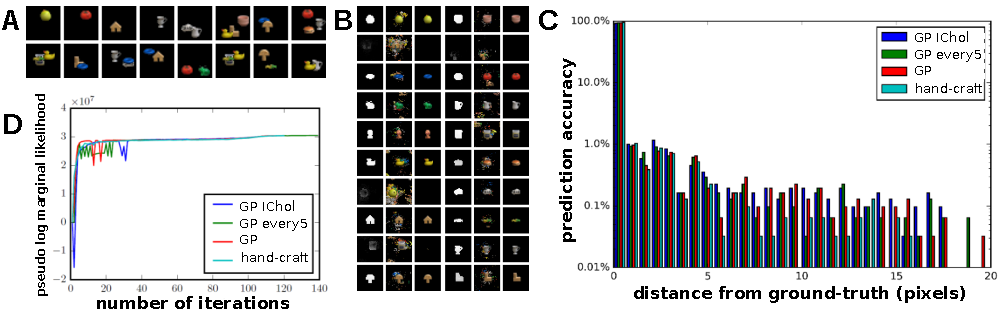
\includegraphics[width=\textwidth]{inveca/invec_mod.pdf}%{figs/inveca/invec_mod.pdf}
%\caption{Results of GP-select on the Translation Invariant model.
%%%\comm{fix for new experiments -- really great speedup (fivefold from less frequent updates, plus factor of 100 from chol (since it's square in the number of features reduced))}
%\textbf{C} shows the log-scale histogram of the prediction accuracy for all four selection functions in terms of the distance from the predicted location to the ground truth location: GP-select with no modifications (GP), the incomplete Cholesky decomposition (GP IChol), with updated kernel hyperparameters every 5 EM iterations (GP every5), and with hand-crafted selection (hand-craft).
%the $x$-axis shows the distance from the ground-truth location in terms of pixels, and the $y$-axis shows the percentages.
%\textbf{D} shows the convergence of the pseudo log likelihood [of the model parameters learned at each EM iteration] for the both selection functions over all EM iterations. 
%Figures \textbf{C} and \textbf{D} show the equivalent accuracy/performance of inference with all GP-select functions versus the hand-crafted selection function.
%'GP IChol' represents a factor of $100$ speedup vs. 'GP', and 'GP every5' represents a factor of $5$ speedup.
%}
%\label{fig:inveca}
%\end{center}
%\end{figure*}

Now that we have verified that GP-select can be applied to various generative graphical models and converge to ground-truth parameters, we consider a more challenging model that addresses a problem in computer vision: \emph{translations of objects in a scene}.

\textbf{Model.}
%
\rev{Translation invariant models address the problem that, e.g., visual objects can appear in any location of an image. Probabilistic models for translation invariance are particularly appealing as they allow to separately infer object positions and object type, making them very interpretable and powerful tools, e.g., for image processing.}

\rev{However,} translation invariant models are particularly difficult to optimize because they must consider a massive latent variable space: evaluating multiple objects and locations in a scene leads a \textit{latent space complexity of the number of locations exponentiated by the number of objects}.
% --- Hand-crafted pre-selections have been successfully applied to translational invariant models.
%Especially considering multiple objects in a scene, the complexity of latent space becomes the number of locations to the power of the number of objects.
Inference in such a massive latent space heavily relies on the idea of variable selection to reduce the number of candidate objects and locations. In particular, hand-engineered selection functions that consider \emph{translational invariance} have been successfully applied to this type of model~\citep{DaiLucke2012b,DaiLucke2014,DaiEtAl2013}.
%
The selection function used so far for reducing latent space complexity in this model has been constructed as follows.
First, the candidate locations of all the objects in the model are predicted.
Then a subset of candidate objects that might appear in the image are selected according to those predicted locations.  
Next, the subset of states $\Kn$ is constructed 
\rev{according to the combinations of the possible locations and numbers of candidate objects}.
% --- Then the true posterior probabilities are estimated for this preselected latent subspace, while considering the posterior probabilities in the rest space to be zero.
The posterior distribution is then computed following Equation~\eqref{eq:sel-post}.

This selection system is very costly: the selection function has parameters which need to be hand-tuned, e.g., the number of representative features, and %, which leads to problems when this number is either too big or too small.
it needs to scan through the entire image, considering all possible locations, which becomes computationally demanding for large-scale experiments.
%
%In this experiment, we follow a similar design to use a GP regression model as a general selection. Different from the applications in previous models,
To maximally exploit the capabilities of the GP-selection function, we directly use the GP regression model to \textit{predict the possible locations} of a component \textit{without introducing any knowledge of translation invariance} into the selection function. In this work, a GP regression model is fitted from the input image to marginal posterior probabilities of individual components appearing at all possible locations. Therefore, the input to the GP-selection function is the image to be inferred and the output is a score for each possible location of each component in the model.
For example, when learning $10$ components in a $D=30\times 30$ pixel image patch, the output dimensionality of GP-select is $9000$.
This task is computationally feasible, since GP models scale linearly with output dimensionality.
The inference of components' locations with GP-select is significantly faster than the selection function in the original work, as it avoids explicitly scanning through the image.

Although there are additional computations necessary for an automatic selection function like GP-select, for instance due to the adjustment of its parameters,  %Unfortunately, the computation of updating the parameters of a GP regression model is relatively expensive. 
there are many options to reduce computational costs. %reducing the cost of the parameter fitting. 
First, we may approximate the full $N \times N$ Gram matrix by an incomplete Cholesky approximation~\citep{FinSch01} 
resulting in a cost of $O(N\times Q)$, where $Q << N$ is the rank of the Cholesky approximation.
% XXX
% XXX
%
%We follow the approach of \cite{FinSch01}
%\citep[][section 5]{SonGreBicLowGue11} 
%for the low-rank approximation of the inversion of covariance matrix (incomplete Choleksy decomposition). 
Second, we may reduce the frequency of kernel hyperparameter updates to only every $T\ast*$ EM iterations, where a $T\ast* > 1$ represents a corresponding computation reduction.
% to correspondingly reduce the average time by a factor of $5$.
The combination of the Cholesky approximation plus infrequent updates will have the following benefits: a factor of five speedup for infrequent updates, and a factor of $(N-Q)^2$ speedup from incomplete Cholesky, where $Q$ is the rank of the Cholesky approximation and $N$ is the number of original data points. 

%Intuitively, using GP-select for this problem makes sense, as objects are typically not uniformly distributed in a scene and with limited  observations we often can give a good rough prediction of object locations.
%Approaches such as data-driven location are based entirely on this idea, going further to convert a detection problem into an information retrieval problem, and recently achieving the state-of-art performance on object detection \citep{Rodriguez-SerranoL13}.

\textbf{COIL Dataset.}
%
\begin{figure*}[t!]%[ht]
\centering
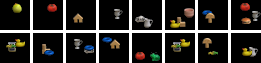
\includegraphics[width=1\textwidth]{inveca/dataSamples.png}%{figs/inveca/invec_mod.pdf}
\caption{COIL Dataset \citep{coil100}: 
A handful of data points used in experiments with the Translation Invariant Occlusive (InvECA) model, showing the occluding objects to be learned.
}
\label{fig:inveca-data}
\end{figure*}
%
We apply our GP-selection function to the \emph{Invariant Exclusive Component Analysis (InvECA) model}~\citep{DaiLucke2012b,DaiEtAl2013}.
For our experiments, we consider an image dataset used in previous work: data were generated using objects from the COIL-100 image dataset \citep{coil100}, taking $16$ different objects, downscaled to $D=10 \times 10$ pixels and segmented out from the black background.
A given image was generated by randomly selecting a subset of the $16$ objects, where each object has a probability of $0.2$ of appearing.
The appearing objects were placed at random positions on a $30 \times 30$ black image.
When the objects overlap, they occlude each other with a different random depth order for each image.
In total, $N=2000$ images were generated in the dataset (examples shown in Figure~ \ref{fig:inveca-data}).%\ref{fig:inveca}\textbf{A}).

The task of the InvECA model is to discover the visual components (i.e. the images of $16$ objects) from the image set without any label information. 
We compare the visual components learned by using \emph{four different selection functions in the InvECA model}: the hand-crafted selection function used in the original work by ~\citet{DaiLucke2012b}, GP-select updated every iteration, GP-select updated every $T*=5$ iterations, and GP-select with incomplete Cholesky decomposition updated every iteration, or $T\ast=1$ (in this manner we isolate the improvements due to Cholesky from those due to infrequent updates). 
In these experiments, the parameters of GP-select are optimized at the end of each $T*$ EM iteration(s), using a maximum of $20$ gradient updates.
The number of objects to be learned is $H=20$ and the algorithm pre-selects $H'=5$ objects for each data point.
%there were $H'=5$ preselected objects.
The kernel used was the composition kernel, as suggested in Section 4.1, although after fitting the hyperparameters only the RBF kernel remained with large variance (i.e. a linear kernel alone would not have produced good variable selection, thus the flexible composition kernel was further shown to be a good choice).

\textbf{Results.}
%The results are shown in Figure~\ref{fig:inveca}. 
%
\begin{figure*}[t!]%[ht]
\centering
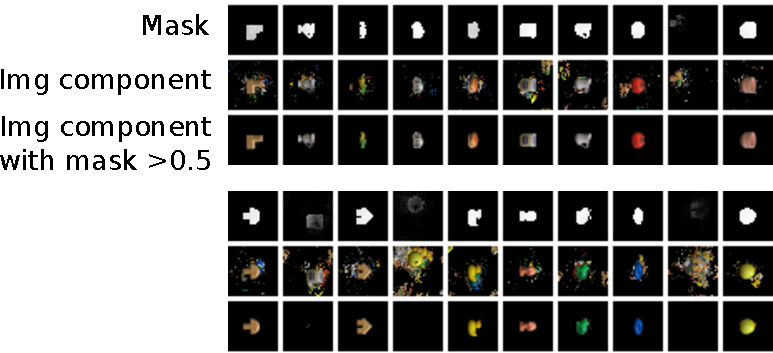
\includegraphics[width=\textwidth]{inveca/params_j_2blocks.pdf}%{figs/inveca/invec_mod.pdf}
\caption{Image components and their masks learned by GP-select with the Translation Invariant model. GP-select learned all objects in the dataset.
The first row shows the mask of each component, %/ object / feature, 
the second row shows the learned image components, % feature representations %/ object, 
and the third row shows only the area of the learned components that had a mask $>0.5$.
\rev{For the second three-row block of images, the same titles of the first three-row block hold.}
}
\label{fig:inveca-params}
%\end{center}
\end{figure*}
%
All four versions of the InvECA model using each of the selection functions considered successfully recover each individual objects in our modified COIL image set. 
The learned object representations with GP-select are shown in Figure~\ref{fig:inveca-params}. %\textbf{B}.
Four additional components developed into representations, however these all had very low mask values, allowing them to easily be distinguished from other true components.

\begin{figure}[ht!]%[ht]
\centering
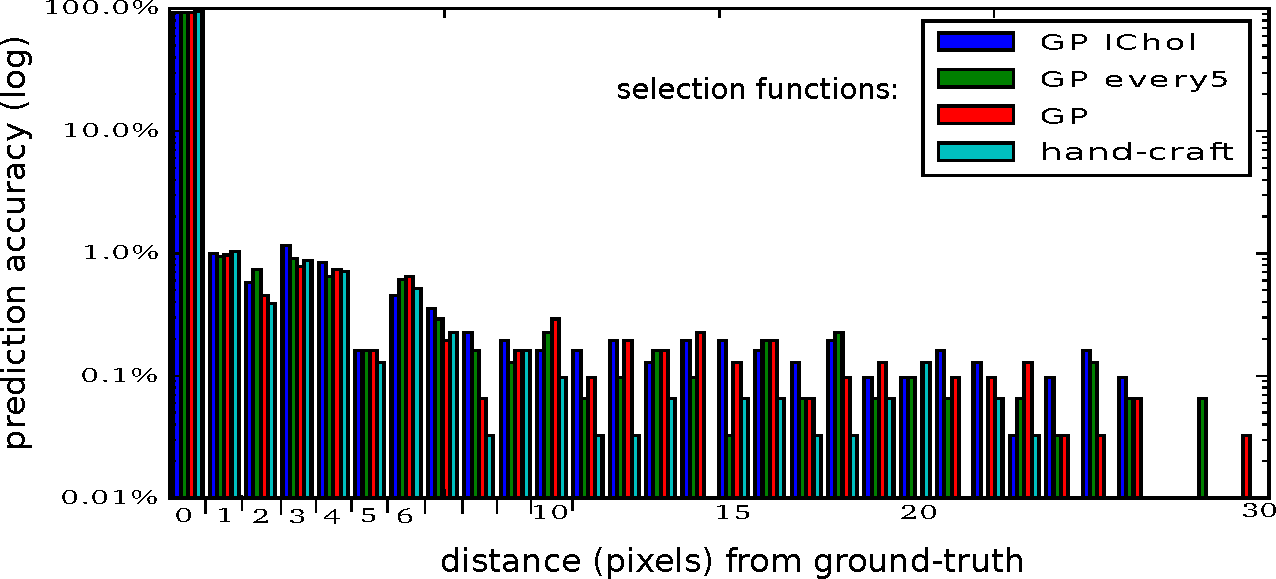
\includegraphics[width=\textwidth]{inveca/locationHist_js.pdf}%{figs/inveca/invec_mod.pdf}
\caption{Prediction accuracy of the four selection functions in the InvECA model.
%%%\comm{fix for new experiments -- really great speedup (fivefold from less frequent updates, plus factor of 100 from chol (since it's square in the number of features reduced))}
Functions depicted in the figures: GP-select with no modifications (GP, red), the incomplete Cholesky decomposition (GP IChol, blue), with updated kernel hyperparameters every 5 EM iterations (GP every5, green), and with hand-crafted selection (hand-craft, cyan).
Shown: the log-scale histogram of the prediction accuracy for the four selection functions, measured by the distance each function's predicted object location was to the ground-truth object location. 
All bars of the selection functions show very similar accuracy for the various distances. 
}
\label{fig:inveca1}
%\end{center}
\end{figure}
%
\begin{figure}[ht!]%[ht]
\centering
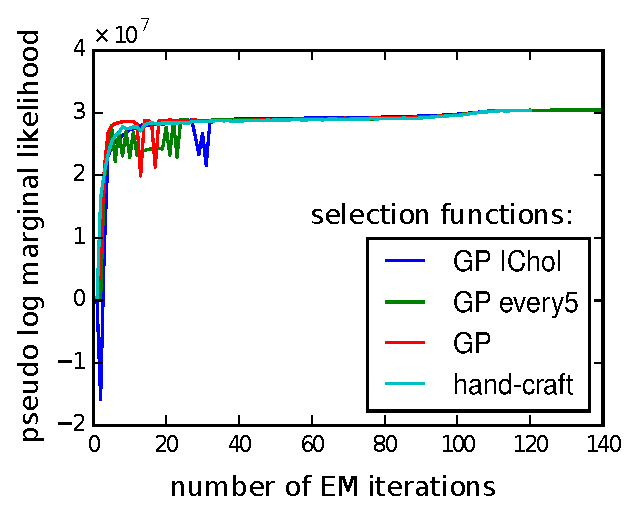
\includegraphics[width=.6\textwidth]{inveca/inveca_L_js.pdf}%{figs/inveca/invec_mod.pdf}
\caption{Baseline comparison of the four selection functions in the InvECA model.
%%%\comm{fix for new experiments -- really great speedup (fivefold from less frequent updates, plus factor of 100 from chol (since it's square in the number of features reduced))}
Functions depicted in the figures are identical to those in Figure~\ref{fig:inveca1}.
%
Shown: the convergence of the pseudo log marginal likelihood [of the model parameters learned at each EM iteration] for the four selection functions over all EM iterations. After about 40 EM iterations, all selection function versions of the algorithm converge to the same likelihood solution.  
Simultaneously, the GP-select approaches exhibit no loss of accuracy compared to the hand-crafted function,  and 
'GP IChol' represents a factor of $100$ speedup vs. 'GP', and 'GP every5' represents a factor of $5$ speedup.
}
\label{fig:inveca2}
%\end{center}
\end{figure}
%
Next, we compare the accuracy of the four selection functions.
For this, we collected the object locations (pixels) indicated by each selection function after all EM iterations, 
applied the selection functions (for the GP selection functions, this was using the final function learned after all EM iterations) to the entire image dataset again, 
then compared these results with the ground-truth location of all of the objects in the dataset.
%the GP-select approach, 
% XXX this sentence made no sense to me, so i guessed what zhenwen meant:
%we collected the GP-selection after learning, and applied the GP selection function to the whole dataset again, then compared with the ground-truth location of all the objects in the datasets.
%
%
The accuracy of the predicted locations was then computed by comparing the distance of all ground-truth object location to the location of the top candidate locations from each selection function. % and the ground-truth location. 
 See Figure~\ref{fig:inveca1} for a histogram of these distances and the corresponding accuracy for all selection functions. Note that the percentages in the histogram are plotted in log scale.
%
%
%XXX
\iffalse
\begin{figure}[ht!]%[ht]
\centering
\includegraphics[width=\textwidth]{inveca/accuracy.pdf}%{figs/inveca/invec_mod.pdf}
\caption{Accuracy of the four selection functions in the Translation Invariant model.
%%%\comm{fix for new experiments -- really great speedup (fivefold from less frequent updates, plus factor of 100 from chol (since it's square in the number of features reduced))}
Functions depicted in the figures: GP-select with no modifications (GP, red), the incomplete Cholesky decomposition (GP IChol, blue), with updated kernel hyperparameters every 5 EM iterations (GP every5, green), and with hand-crafted selection (hand-craft, cyan).
\textbf{A} The log-scale histogram of the prediction accuracy for the four selection functions, measured by the distance each function's predicted object location was to the ground-truth object location. 
All bars of the selection functions show nearly equivalent accuracy for the various distances. 
%the $x$-axis shows the distance from the ground-truth location in terms of pixels, and the $y$-axis shows the percentages.
\textbf{B} The convergence of the pseudo log marginal likelihood [of the model parameters learned at each EM iteration] for the selection functions over all EM iterations. 
}
\label{fig:inveca}
%\end{center}
\end{figure}
%
%
\begin{figure}[ht!]
\ContinuedFloat
\centering
\caption{After about 40 EM iterations, all four selection function versions of the algorithm converged to the same likelihood. Both figures show equivalent performance of the GP-select approaches with the hand-crafted function, but 
%show that the accuracy/performance of inference with all GP-select functions is equivalent to the hand-crafted selection function.
'GP IChol' represents a factor of $100$ speedup vs. 'GP', and 'GP every5' represents a factor of $5$ speedup.}
% \lipsum[4-8]

% \smallskip
% \hrule % consider using a visual separator between float material and running text
\end{figure}
\fi
%
%Furthermore, the pseudo log likelihood \cite{DaiEtAl2013} for both selection functions are shown in Figure~\ref{fig:inveca}\textbf{D}.
%=======
Also, as a baseline verification, 
%we also estimated the prediction accuracy of the original selection function by computing the pseudo log likelihood \cite{DaiEtAl2013}.
%
we computed and compared the pseudo log likelihood \citep{DaiEtAl2013} of the original selection function to the three GP-select based ones.
% 
The pseudo log likelihood for all selection functions is shown in Figure~\ref{fig:inveca2}.
Figures~\ref{fig:inveca1}-\ref{fig:inveca2} show that all four selection functions can very accurately predict the locations of all the objects in the dataset -- 
the GP-select selection functions yields no loss in inference performance in comparison to the original hand-engineered selection function. 
Even those using speed-considerate approximations (incomplete Cholesky decomposition of the kernel matrix (GP IChol) and updating kernel hyperparameters only every 5 EM iterations (GP every5)) have indistinguishable prediction accuracy on the task.

%\textbf{Scalability.}

An analysis of the benefits indicate that, as GP-select avoids explicitly scanning through the image, the time to infer the location of an object is significantly reduced compared to the hand-crafted function. GP-select requires $22.1$ seconds on a single CPU core to infer the locations of objects across the whole image set, while the hand-crafted function requires $1830.9$ seconds. In the original work, the selection function was implemented with GPU acceleration and parallelization. 
Although we must compute the kernel hyperparameters for GP-select, 
%which necessitates strategies for reducing computational cost.
it is important to note that the hyperparameters need not be fit perfectly each iteration -- for the purposes of our approach, a decent approximation suffices for excellent variable selection. 
 In this experiment, updating the parameters of GP-select with $10$ gradient steps took about $390$ seconds for the full-rank kernel matrix. 
When we compute the incomplete Cholesky decomposition while inverting the covariance matrix, compute time was reduced to $194$ seconds (corresponding to the $(N-Q)^2$ speedup, where $Q$ is the rank of the Cholesky approximation), with minimal loss in accuracy.
Furthermore, when updating the GP-select hyperparameters only every 5 iterations, average compute time was reduced by another one fifth, again without loss in accuracy.


% potential extension multiple output GP.
% cascade prediction

\section{Discussion}
\label{disc}
%
% XXX changed score to selection
We have proposed a means of achieving fast EM inference in Bayesian generative models, by
learning an approximate selection function to determine relevant latent variables
for each observed variable. The process of learning the relevance functions
is interleaved with the EM steps, and these functions
are used in obtaining an approximate posterior distribution in the subsequent EM iteration.
The functions themselves are learned via Gaussian process regression,
and do not require domain-specific engineering, unlike previous selection functions.
In experiments on mixtures and sparse coding models with interpretable output,
the learned selection functions behaved in accordance with our expectations for the posterior
distribution over the latents.  

The significant benefit we show empirically is that by learning the selection function in a general and flexible nonparametric way, we can avoid using potentially expensive hand-engineered selection functions.
Cost reduction is both in terms of required expertise in the problem domain, and computation time in identifying the relevant latent variables.
Inference using our approach required 22.1 seconds on a single CPU core, versus  1830.9 seconds with the original hand-crafted function 
for the complex hierarchical model of \citep{DaiEtAl2013}.

A major area where further performance gains might be expected is in
improving computational performance, since we expect the greatest
advantages of GP-select to occur for complex models at large scale. For instance,
 kernel ridge regression may be parallelized \citep{zhang14divide},
or the problem may be solved in the primal via random Fourier features \citep{LeSarSmo13}.
Furthermore, there are many recent developments regarding the scaling up of GP inference to large-scale problems, e.g., sparse GP approximation
~\citep{sparseGP}, stochastic variational inference \citep{HensmanEtAl2013,Hensman2012}, using parallelization techniques and GPU acceleration \citep{DaiEtAl2014}, or in combination with stochastic gradient descent~\citep{Bottou08thetradeoffs}. 
%XXX new rebuttals:
For instance, for very large datasets where the main model is typically trained with mini-batch learning, stochastic variational inference can be used for GP fitting as in \citep{HensmanEtAl2013} and the kernel parameters can be efficiently updated each (or only every $T*$ few) iteration with respect to a mini-batch.



\iffalse
\subsubsection*{Acknowledgements}
We acknowledge funding by the German Research Foundation (DFG) under grants LU 1196/4-2 (JS), LU 1196/5-1 (JL), by the Cluster of Excellence EXC 1077/1 "Hearing4all" (JL), and by the RADIANT and WYSIWYD (EU FP7-ICT) projects (ZD).
\fi

% XXX depending on submission target:
%\bibliography{cnml-all.bib}
%\bibliographystyle{icml2015}



% XXX
%The increase generality and flexibility of GP selection does not come without any cost, however.
%Depending on the used kernel, the computational demand for GP selection can scale polynomial with the number of data points (HI GUYS PLEASE VERIFY THIS and add if cubic or quadratically) while most previously used selection functions scale linearly. By coupling selection function learning to GPs, any improvements for GP inference and learning can directly be leveraged, however.
%Ongoing research for efficient GP classification investigates, for instance, NOW NAME APPROACHES HERE - ARTHUR, ZHENWEN?
%
%AG
%Furthermore, given complex graphical models, GP selection could be applied to help guide the design of more efficient but model specific selection functions, or to validate such functions. The experiments presented here could, for instance, also be interpreted as a validation of the selection functions used in previous work.
%
%Smaller-scale applications can be used for comparison of model specific selection functions and GP selection as discussed here; efficient model specific selection function defined using GPs could then be used for large-scale applications.

%Current work is applying the GP inference approach to complex models at large-scale, where we expect to the benefits of this approach to shine -- both in terms of computational efficiency as well as the flexibility offered by such a simple regression approach to "pre-learn" complicated inference landscapes.
% - approximate GP regression -- subset of data to compute kernel matrix?
% - low rank approx to kernel matrix?
% - optimize kernel parameters on a less-frequent schedule .. i.e. based on how much the parameters changed the last times it optimized
% - don't compute regression every EM iteration -- use the same regression from previous iterations when the predictive covariance is "low enough" ... but then "low enough" needs to be defined

% % OLD discussion
% Results so far are promising -- the Gaussian mixture model demonstrated that data exist for which a linear predictor will always fail at finding relevant features, whereas a nonlinear predictor offers flexibility without a priori assumptions.
% The results on diverse sparse coding models also demonstrate the power of the approach in its ability to learn selection functions
% hand-engineered selection functions even via simple linear regression.
% Current work is applying this inference approach to complex models at large-scale, where we expect to the benefits of this approach to shine -- both in terms of computational efficiency as well as the flexibility offered by such a simple regression approach to "pre-learn" complicated inference landscapes.
% Considering the translational invariant exclusive model, the pre-selection consists of two steps: first, selecting a small of candidate positions for each component in the model, and then selecting a small set of candidate components.

% The GP-selection approach lends itself to many possible ways of being applicable at larger scale, which is a topic of ongoing research. Mention ideas to scale up??
% - approximate GP regression -- subset of data to compute kernel matrix?
% - low rank approx to kernel matrix?
% - optimize kernel parameters on a less-frequent schedule .. i.e. based on how much the parameters changed the last times it optimized
% - don't compute regression every EM iteration -- use the same regression from previous iterations when the predictive covariance is "low enough" ... but then "low enough" needs to be defined
